\documentclass[nolayout]{article}

\usepackage[utf8]{inputenc}
\usepackage[english]{babel}
\usepackage{amsmath,amsthm}
\usepackage{geometry}
\usepackage[textwidth=4cm,textsize=footnotesize]{todonotes}
\usepackage{fancyhdr}
\pagestyle{fancy}
\usepackage{amssymb,color,bbm,xargs}
\usepackage{graphicx}
\usepackage[active]{srcltx}
\usepackage{ifthen}
\usepackage{enumerate}
\usepackage{color}
\usepackage{accents}
\usepackage{dsfont}
\usepackage[ruled,vlined]{algorithm2e}
\usepackage{subfig}
\usepackage{multirow}
\usepackage{placeins}

\usepackage{aliascnt}
\theoremstyle{plain}
\newtheorem{theorem}{Theorem}
\newtheorem{assumption}{H\hspace{-3pt}}
\newtheorem*{assumption*}{A}
\newtheorem{assumptionDelta}{H\hspace{-3pt}(\Delta)}
\newtheorem{assumptionsmallSetD}{H\hspace{-3pt}(\smallSetD \times \smallSetD)}
\newtheorem{assumptionAR}{AR\hspace{-3pt}}
\newtheorem{assumptionCN}{CN\hspace{-3pt}}


\newaliascnt{proposition}{theorem}
\newtheorem{proposition}[proposition]{Proposition}
\aliascntresetthe{proposition}

\newaliascnt{lemma}{theorem}
\newtheorem{lemma}[lemma]{Lemma}
\aliascntresetthe{lemma}
\newaliascnt{corollary}{theorem}
\newtheorem{corollary}[corollary]{Corollary}
\aliascntresetthe{corollary}

\newtheorem{hypothese}{Hypothesis}
\newtheorem{fact}[theorem]{Fact}


\theoremstyle{definition}
\newaliascnt{definition}{theorem}
\newtheorem{definition}[definition]{Definition}
\aliascntresetthe{definition}

\newaliascnt{remark}{theorem}
\newtheorem{remark}[remark] {Remark}
\aliascntresetthe{remark}



\usepackage{hyperref}
\usepackage[nameinlink,noabbrev]{cleveref}

\providecommand*{\definitionautorefname}{Definition}
\providecommand*{\lemmaautorefname}{Lemma}
\providecommand*{\exampleautorefname}{Example}
\providecommand*{\propositionautorefname}{Proposition}
\providecommand*{\procautorefname}{Procedure}
\providecommand*{\exerciseautorefname}{Exercise}
\providecommand*{\corollaryautorefname}{Corollary}
\providecommand*{\remarkautorefname}{Remark}
\providecommand*{\algorithmautorefname}{Algorithm}
\providecommand*{\assumptionautorefname}{H\hspace*{-3pt}}  
\providecommand*{\assumptionARautorefname}{AR\hspace*{-3pt}}
\providecommand*{\assumptionCNautorefname}{CN\hspace*{-3pt}}


\newcommand*{\largedot}{\cdot}

\def\Rset{\mathbb{R}}
\def\Nset{\mathbb{N}}
\def\nset{\mathbb{N}}
\def\rset{\mathbb{R}}
\def\varb{b}
\newcommand{\1}{\mathbbm{1}}

\newcommand{\floor}[1]{\left\lfloor #1 \right\rfloor}
\newcommand{\ceil}[1]{\left\lceil #1 \right\rceil}

\def\ie{\textit{i.e.}}
\newcommand{\coint}[1]{\left[#1\right)}
\newcommand{\ocint}[1]{\left(#1\right]}
\newcommand{\ooint}[1]{\left(#1\right)}
\newcommand{\ccint}[1]{\left[#1\right]}
\newcommand{\Wienerspace}{\mathbf{W}}

\def\PE{\mathbb{E}}
\newcommandx{\PEt}[2][1=]{\mathbb{E}_{#1}\left[#2\right]}
\def\rmd{\mathrm{d}}
\def\rme{\mathrm{e}}
\def\target{\pi}
\def\dim{d}
\def\score{\accentset{\largedot}{\ell}}
\def\Vdot{\dot{V}}
\def\unitarget{f}
\def\rmL{\mathrm{L}}
\def\dimy{\mathsf{p}}
\def\dimz{\mathsf{m}}
\def\bfX{\boldsymbol{X}}
\def\xbf{\boldsymbol{x}}
\def\ybf{\boldsymbol{y}}
\def\Xbf{\boldsymbol{X}}
\def\G{\mathcal{G}}
\def\barG{\overline{G}}
\def\barH{\overline{H}}
\def\Gammabf{\mathbf{\Gamma}}
\def\Ybf{\boldsymbol{Y}}
\newcommand{\norm}[1]{\left\Vert #1 \right \Vert}
\newcommand{\plusinfty}{+ \infty}
\newcommand{\defEns}[1]{\left \{ #1 \right \}}
\newcommand{\abs}[1]{\left\vert #1 \right\vert}
\def\Zbf{\boldsymbol{Z}}
\def\eqsp{\,}
\def\leb{\lambda}
\def\limd{\underset{d\to +\infty}{\longrightarrow}}
\newcommand{\normMat}[2]{\left\|#2\right\|_{#1}}



\newcommand{\parenthese}[1]{\left( #1 \right)}
\newcounter{hypH}
\newenvironment{hypH}{\refstepcounter{hypH}\begin{itemize}
\item[{\bf H\arabic{hypH}}]}{\end{itemize}}
\newcommand{\eqdef}{\ensuremath{:=}}
\newcommand{\setAccept}{\mathcal{A}}
\def\iid{\operatorname{i.i.d.}}
\newcommand{\sachant}[1]{\left| #1 \right.}
\newcommand{\setDisconDotV}{\mathcal{D}_{\dot{V}}}

\def\restriction#1#2{\mathchoice
              {\setbox1\hbox{${\displaystyle #1}_{\scriptstyle #2}$}
              \restrictionaux{#1}{#2}}
              {\setbox1\hbox{${\textstyle #1}_{\scriptstyle #2}$}
              \restrictionaux{#1}{#2}}
              {\setbox1\hbox{${\scriptstyle #1}_{\scriptscriptstyle #2}$}
              \restrictionaux{#1}{#2}}
              {\setbox1\hbox{${\scriptscriptstyle #1}_{\scriptscriptstyle #2}$}
              \restrictionaux{#1}{#2}}}
\def\restrictionaux#1#2{{#1\,\smash{\vrule height .8\ht1 depth .85\dp1}}_{\,#2}}

\newcommandx\sequence[3][2=,3=]
{\ifthenelse{\equal{#3}{}}{\ensuremath{\{ #1_{#2}\}}}{\ensuremath{( #1_{#2}, \eqsp #2 \in #3 )}}}
\newcommandx{\sequencen}[2][2=n\in\nset]{\ensuremath{( #1, \eqsp #2 )}}
\newcommandx\dsequence[4][3=k,4=\zset]{\ensuremath{( (#1_{#3}, #2_{#3}), \eqsp #3 \in #4 )}}
\newcommandx{\as}[1][1=\PP]{\ensuremath{#1\--\mathrm{a.s.}}}
\newcommand{\eqspp}{\ \ }

\def\canonicalFiltration{\mathscr{B}}

\def\tildeX{\widetilde{X}}
\def\tildeY{\widetilde{Y}}
\def\barX{\bar{X}}
\def\barY{\bar{Y}}
\def\barS{\bar{S}}
\newcommand{\coupling}[2]{\mathcal{C}(#1,#2)}
\newcommand\proba[1]{\mathbb{P}\left[ #1 \right]}
\newcommand\expe[1]{\mathbb{E}\left[ #1 \right]}
\def\osc{\operatorname{osc}}
\def\borel{\mathcal{B}}
\def\mcf{\mathcal{F}}
\begin{document}

\title{Rao-Blackwellised Two-filter algorithm for Conditionally Linear and Gaussian models}
\date{}

\author{Ngoc Minh Nguyen\footnote{LTCI, CNRS and T\'el\'ecom ParisTech, 46 rue Barrault 75634 Paris Cedex 13, France.}, Sylvain {L}e {C}orff\footnote{Laboratoire de Math\'ematiques d'Orsay, Univ. Paris-Sud, CNRS, Universit\'e Paris-Saclay, 91405 Orsay, France.} and Eric Moulines\footnote{Centre de Math\'ematiques Appliqu\'ees, UMR 7641, Ecole Polytechnique, France.}}

\lhead{Ngoc Minh Nguyen et al.}
\rhead{Conditionally Linear and Gaussian models}

\maketitle

\begin{abstract}
This paper focuses on Sequential Monte Carlo based approximations of smoothing distributions in conditionally linear and Gaussian state spaces. Only a few methods have been proposed to reduce Monte Carlo variance of smoothers with Rao Blackwellisation steps for these models. The most widely used Rao Blackwellised Sequential Monte Carlo smoothers introduced in \cite{kim:1994,lindsten:bunch:sarkka:schon:godsill:2015,sarkka:bunch:godsill:2012,lindsten:bunch:godsill:schon:2013} are based on the Forward Backward decomposition of the marginal smoothing distribution. In \cite{kim:1994}, a structural approximation of the model is used to simplify the backward pass while \cite{lindsten:bunch:sarkka:schon:godsill:2015,sarkka:bunch:godsill:2012,lindsten:bunch:godsill:schon:2013} use Rao Blackwellisation steps without any approximation in both forward and backward passes. In this paper, these algorithms are compared to an extension of the Two-filter based algorithm of \cite{briers:doucet:maskell:2010} with additional explicit Rao Blackwellised steps to improve its performance. The procedures are applied to commodity markets which are described using a two factor model based on the spot price and a convenience yield. Parameters are estimated using  an Expectation Maximization and the performance of the proposed procedure is assessed with Chicago Mercantile Exchange crude oil data.


%In this paper, commodity markets are described using a two factor model based on the spot price and a convenience yield representing the benefit or cost required for holding the physical commodity. It is assumed that the market structure has different regimes which depend on existing stocks and contracts or other externalities. These different regimes are modeled using a finite state space unobserved Markov chain, each regime corresponding to an  equilibrium behavior of the spot price and the convenience yield. At each time step, it is assumed that noisy observations of future contracts are available which leads to represent commodity markets dynamics using a conditionally linear and Gaussian state space model. We propose a new algorithm to approximate the conditional distributions of the states (spot, convenience yield and regime indicator) given a set of observations. These approximations are obtained combining Sequential Monte Carlo methods and Kalman smoothing techniques  and may be used to detect significant regime switching times and to estimate model parameters with an Expectation Maximization based algorithm. The performance of the proposed procedure is assessed with Chicago Mercantile Exchange crude oil data.
\end{abstract}

\section{Introduction} \label{sec:intro}
%Modeling commodity prices is a crucial step to valuate contingent claims related to energy markets and to optimize storage or extraction strategies. In \cite{gibson:schwartz:1990,schwartz:1997}, the authors proposed a model where the spot price of a commodity$(S_t, t \geq 0)$ depends on a second factor $(\delta_t, t \geq 0)$, referred to as the instantaneous convenience yield. This factor plays the role of dividends in equity markets and models the benefit of holding the physical commodity or the storage and maintenance costs required to keep the commodity. In this model, this convenience yield is described as an Ornstein-Uhlenbeck process:
%\begin{align*}
%\rmd S_{t} & = (r-\delta_{t})S_{t}\rmd t+\sigma S_{t} \rmd W_{t}^{1} \eqsp,\\
%\rmd \delta_{t} & = \kappa(\alpha-\delta_{t})\rmd t+\eta \rmd W_{t}^{2} \eqsp, \quad \rmd \langle W_t^1, W_t^2\rangle = \rho \rmd t\eqsp,
%\end{align*}
%where the parameter $\left(r, \sigma, \kappa, \alpha, \eta, \rho \right)$ are constant and $( (W_t^1,W_t^2), t \geq 0)$ are standard Brownian motions under the historical probability $\mathbb{P}$. A similar model may be written under the risk-neutral probability $\mathbb{Q}$ with an obvious transformation of the parameters. This convenience yield based model has been extended in \cite{casassus:colin:dufresne:2005,liu:tang:2011}. In this model, the convenience yield is meant to revert to its equilibrium value $\alpha$ at speed $\kappa$. 
%
%
%This model appear to be too restrictive as energy markets are not likely to revert to a single equilibrium value. This assumption is relaxed using Markov switching models to allow several possible regimes for the spot price and the convenience yield. The regime switching autoregressive model introduced in \cite{hamilton:1988,hamilton:1989} for the term structure of interest rates has been generalized by \cite{kim:1994} to general state-space models. This Markov switching model also extends the dynamic linear model of \cite{shumway:stoffer:1991} by using a time dependent switching process and introducing regime changes in the observation model. Regime switching models based on an unobserved Markov chain have been widely used to represent commodity prices, see for instance \cite{fong:see:2002} for crude oil data or \cite{mount:ning:cai:2006} for electricity prices. See also \cite{naifar:dohaiman:2013} for a two-regime model (crisis regime and non-crisis regime) to obtain the evidence of a significant correlation between crude oil prices and short-term interest rate during the financial crisis. In \cite{chiarella:clewlow:kang:2009}, a two-factor model for the gas forward price is introduced to model where the parameters of the volatility function may change depending on the market structure. In order to capture gas price dynamics, \cite{chen:forsyth:2010} proposed a single factor model for the crude oil spot price using a mean reverting process with two equilibrium levels. Following \cite{almansour:2016}, the spot price and convenience yield are described in this paper as:
%\begin{align*}
%\rmd S_{t} & = (r-\delta_{t})S_{t}\rmd t+\sigma_{a_t} S_{t}\rmd W_{t}^{1} \eqsp,\\
%\rmd\delta_{t} & = \kappa_{a_t}(\alpha_{a_t} -\delta_{t})\rmd t+\eta_{a_t} \rmd W_{t}^{2} \eqsp, \quad \rmd\langle W_t^1, W_t^2\rangle = \rho_{a_t} \rmd t\eqsp,
%\end{align*}
%where $(a_t)_{t\ge 0}$ is a finite state space Markov process. 
%
%This model allows to exhibit fundamental features of commodity future prices, which typically display different regimes of volatility and/or convenience yield. A two-regime model is already sufficient to produce stylized effects such as contango (increase of future prices) and backwardation (decrease of future prices).  


%Assuming that the switching rate between regimes is small compared to the inverse of the discretization period, the discretized version of the spot price and convenience yield $Z_k= (\ln S_k, \delta_k)$ (the sampling period is taken to be 1) is modeled as a 
State space models are bivariate stochastic processes $\{(Y_k,Z_k)\}_{k\ge 1}$ where the state sequence $\{Z_k\}_{k\ge 1}$ is a Markov chain which is only partially observed through the sequence $\{Y_k\}_{k\ge 1}$. Conditionally on the state sequence $\{Z_k\}_{k\ge 1}$ the observations are independent and for all $\ell\ge 1$ the conditional distribution of $Y_{\ell}$ given $\{Z_k\}_{k\ge 1}$ depends on $Z_{\ell}$ only. These models are used in a large variety of disciplines such as financial econometrics, biology, signal processing, see \cite{delmoral:2013} and the references therein. In general state space models, bayesian filtering and smoothing problems, i.e. the computation of the posterior distributions of a sequence of states $(Z_{k},\ldots,Z_{p})$ for $1\le k\le p\le \ell$ given observations $(Y_{1},\ldots,Y_{\ell})$, are challenging tasks. Filtering refers to the estimation of the distributions of the hidden state $Z_k$ given the observations $(Y_1,\ldots,Y_k)$ up to time $k$, while fixed-interval smoothing stands for the estimation of the distribution of sequence of states $(Z_{k},\ldots,Z_{p})$ given observations $(Y_{1},\ldots,Y_{\ell})$ with $1\le k\le p<\ell$. These distributions are in particular crucial to infer a sequence of states given the observations, see for instance \cite{thrun:burgard:fox:2005} for Simultaneous Localization and Mapping problems, \cite{barshalom:li:kirubarjan:2001} for target tracking problems or \cite{sarkka:2013,douc:moulines:stoffer:2013} for other applications in engineering, telecommunications... In the case where the state and observation models are linear and Gaussian, the filtering is solved explicitly using the Kalman filter \cite{kalman:1960} while the smoothing problem is solved using either the Rauch-Tung-Striebel smoother \cite{rauch:striebel:tung:1965} or the Bryson-Frazier smoother \cite{}. %Many extensions of these algorithms based on local linearization methods have been proposed for nonlinear dynamical systems such as extended Kalman filters, iterated Kalman filters, Gaussian sum filters or Se... 
This paper focuses on  Conditionally Linear and Gaussian Models (CLGM) given for $k\ge 1$ by:
\begin{equation}
\label{eq:model:state}
Z_k = d_{a_{k}} + T_{a_{k}}Z_{k-1}+H_{a_{k}}\varepsilon_k\eqsp,
\end{equation}
where
\begin{enumerate}[-]
\item $(\varepsilon_k)_{k\ge 1}$ is a sequence of independent and identically distributed (i.i.d.) $\dimz$-dimensional Gaussian vectors with zero mean and identity covariance,
\item $(a_k)_{k\ge 0}$ is a homogeneous Markov chain taking values in a finite space $\{1,\ldots,J\}$.  %$Q$ denotes the transition matrix of this Markov chain and by $\pi$ its initial distribution.
\item $(H_j)_{1\le j\le J}$ are positive-definite matrices.
\item $Z_1$ is a $\dimz$-dimensional Gaussian random with mean $\mu_1$ and variance $\Sigma_1$ and is independent of $(\varepsilon_k)_{k\ge 1}$. 
\end{enumerate}
At each time step $k\ge 0$, the observation $Y_k$ is given by:
\begin{equation}
\label{eq:model:obs}
Y_k = c_{a_k} + B_{a_k}Z_k + G_{a_k}\eta_k\eqsp,
\end{equation}
where
\begin{enumerate}[-]
\item $(\eta_k)_{k\ge 0}$ is a i.i.d. sequence of $\dimy$-dimensional Gaussian vectors, independent of $(\varepsilon_k)_{k\ge 1}$ and $Z_1$.
\item $(G_j)_{1\le j \le J}$ are $\dimy \times \dimy$ positive-definite matrices and $(B_j)_{1\le j \le J}$ are $\dimy \times \dimz$ matrices.
\end{enumerate}
Conditionally Linear and Gaussian models have been widely used, see \cite{sarkka:2013} and the references therein. In this paper, the regime switching approach is applied to Chicago Mercantile Exchange crude oil data (see Section~\ref{sec:numerical:experiments}).

An important feature of these models is that, conditionally on a trajectory $(a_1,\ldots,a_n)$ of indicator variables, both the state equation and the observation equation are linear and Gaussian. To exploit this specific structure, it has been suggested in \cite{chen:liu:2000,doucet:godsill:andrieu:2000} to combine Sequential Monte Carlo (SMC) to sample indicator variables with the Kalman filter leading to Rao Blackwellised Monte Carlo filters. %These SMC methods based on sequential importance sampling and resampling techniques introduced in \cite{handschin:mayne:1969} and \cite{rubin:1987} allow to approximate any sequence of conditional distributions of the hidden states given the observations, see \cite{kitagawa:1987,gordon:salmond:smith:1993}. 
Improvements of these early filtering techniques  have been introduced in \cite{doucet:gordon:krishnamurthy:2001,schon:gustafsson:nordlund:2005}. %These algorithms sample only trajectories of indicator variables associated with importance weights, the corresponding state variables $(Z_1,\ldots,Z_k)$ are marginalized and estimated with a Kalman filter, which is the optimal filter in this case. 
%However, many maximum likelihood based estimation procedures such as  the Expectation Maximization  (EM)  algorithm introduced in \cite{dempster:laird:rubin:1977} require to approximate some marginal smoothing distributions of the states and indicator variables. 
%Several algorithms have been developed to solve the smoothing problem using SMC methods: for instance the Forward Filtering Backward Smoothing algorithm (FFBS), the Forward Filtering Backward Simulation algorithm (FFBSi) and the PArticle-based, Rapid Incremental Smoother (PaRIS)  developed respectively in \cite{kitagawa:1996,huerzeler:kunsch:1998,doucet:godsill:andrieu:2000},  \cite{godsill:doucet:west:2004} and \cite{olsson:westerborn:2015}. 
%,lindsten:schon:2011
%In the forward pass of these algorithms, a Rao Blackwellised particle filter such as \cite{chen:liu:2000} is used to approximate the filtering distributions and the corresponding particles, weights and associated trajectories of means and variances of the Kalman filters are stored.
The use of Rao Blackwellisation to solve the smoothing problem has been proved to be challenging and has received satisfactory solutions only recently. The first forward-backward smoother proposed in the literature \cite{fong:godsill:doucet:west:2002} was not fully Rao Blackwellised as it requires to sample the hidden linear states in the backward pass. An alternative, based on a structural approximation of the model suggested in \cite{kim:1994}, was introduced by \cite{barber:2006} to handle the backward pass.  The first fully Rao Blackwellised SMC smoother which does replace the model XXX was proposed by  \cite{briers:doucet:maskell:2010} and extends the Bryson-Frazier smoother for Gaussian linear state space models using the generalized two-filter formula with Rao Blackwellisation steps for the forward and the backward filters.  This two-filter approach combines a forward and a backward filters which are approximated numerically using SMC and Kalman filtering techniques. More recently, \cite{lindsten:bunch:sarkka:schon:godsill:2015,sarkka:bunch:godsill:2012,lindsten:bunch:godsill:schon:2013} introduced a Rao Blackwellised smoother based on the forward-backward decomposition of the FFBS algorithm with Rao Blackwellisation steps both in the forward and backward time directions. 
%The backward pass samples trajectories of indicator variables backward in time using the particles and weights of the forward pass. 


In \cite{briers:doucet:maskell:2010}, for all $1\le i\le n$, the sampled forward and backward sequences are merged to approximate the posterior distribution of $(a_i,z_i)$. In this paper, we propose to approximate the marginal smoothing distribution of $(a_i,z_i)$ by merging the sampled forward and backward trajectories at times $i-1$ and $i+1$ and integrating out all possible paths between time $i-1$ and time $i$ and between time $i$ and time $i+1$ instead of sampling random variables. This explicit marginalization provides an additional Rao Blackwellisation step and produces more robust approximations. 

The paper is organized as follows. An overview of the proposed Monte Carlo algorithms to estimate the smoothing distributions of the hidden states is presented in Section~\ref{sec:RaoBlackwell}. The performance of all these methods is illustrated in Section~\ref{sec:numerical:experiments} with simulated data. Then, a new model is proposed to explain regime switchings for commodity markets. The parameters of the proposed model are estimated using a Monte Carlo EM algorithm where the required conditional expectations are replaced by their estimates based on the proposed SMC method.  
The performance of the extended Rao-Blackwellised two-filter  algorithm is assessed using simulated data and CME crude oil (WTI) data. Intermediate computations and explicit approximations provided by the algorithm are given in the Appendix.


\section{Rao Blackwellised smoothing algorithms}
\label{sec:RaoBlackwell}
This section details the Sequential Monte Carlo algorithms which can be used to approximate the conditional distribution of the states $(a_1,\ldots,a_n)$ or the marginal distributions of $(a_i,z_{i})$ given the observations $(Y_1,\ldots,Y_n)$. For all $m\,\times\,m$ positive-definite matrix $A$ and  all $z\in\mathbb{R}^{m}$ define
\[
\normMat{A}{z}^2 \eqdef z'A^{-1}z\eqsp.
\]
Let $m_{}(a_{i},z_{i-1};z_i)$ be the probability density of the conditional distribution of $Z_i$ given $(a_{i},Z_{i-1})$ and $g_{}(a_{i},z_{i};y_i)$ be the probability density of the conditional distribution of $Y_i$ given $(a_{i},Z_{i})$:
\begin{align}
\label{eq:definition-m}
m_{}(a_{i},z_{i-1};z_i) & \eqdef \left|2\pi\barH_{a_i}\right|^{-1/2}\exp\left\{-\frac{1}{2}\normMat{\barH_{a_i}}{z_i -d_{a_{i}} -T_{a_{i}}z_{i-1}}^2\right\}\eqsp,\\
\label{eq:definition-g}
g_{}(a_{i},z_{i};y_i) & \eqdef \left|2\pi\barG_{a_i}\right|^{-1/2}\exp\left\{-\frac{1}{2}\normMat{\barG_{a_i}}{y_i - c_{a_i} - B_{a_i}z_{i}}^2\right\}\eqsp,
\end{align}
where
\[
\barG_j \eqdef G_jG'_j\;,\; \barH_{j} \eqdef H_jH'_j\eqsp.
\]
%Maximum likelihood estimation of the parameters using the Expectation Maximization algorithm or gradient ascent algorithms requires to compute the posterior distributions of the states $a_{i-1:i},z_{i-1:i}$  given the observations $Y_{1:n}$, written $\phi^n_{i}(a_{i-1:i},z_{i-1:i})$, which cannot be computed in closed-form (the dependency of $\phi^n_{i}$ on $Y_{1:n}$ is dropped for better clarity). SMC methods provide a class of importance sampling and resampling procedures to approximate $\phi^n_{i}(a_{i-1:i},z_{i-1:i})$. 
All the algorithms considered in this paper are based on forward-backward or two-filter decompositions of the smoothing distributions and share the same forward filter detailed in Section~\ref{sec:forward}.  

\subsection{Forward filter}
\label{sec:forward}
The SMC approximation $p^N_{}(a_{1:i},z_{i}|y_{1:i})$ of $p_{}(a_{1:i},z_{i}|y_{1:i})$ may be obtained using the standard Rao Blackwellised  algorithm given in \cite{chen:liu:2000}. The procedure produces a sequence of trajectories $(a^k_{1:i})_{1\le k \le N}$ associated with importance weights $(\omega^k_{i})_{1\le k \le N}$ used to define the following approximation of $p_{}(a_{1:i},z_{i}|y_{1:i})$:
\[
p^N_{}(a_{1:i},z_{i}|y_{1:i}) = \sum_{k=1}^N\delta_{a^k_{1:i}}(a_{1:i})\,\omega^k_{i}\,p_{}(z_{i}|a^k_{1:i},y_{1:i})\eqsp.
\]
In this equation, the conditional distribution of the hidden state $z_{i}$ given the observations $y_{1:i}$ and a trajectory $a^k_{1:i}$ is a Gaussian distribution whose mean $\mu^k_{i}$ and variance $P^k_{i}$ may be obtained by running a Kalman filter as follows. 
\paragraph{Initialization}
At time $i=1$, $(a^k_1)_{1\le k \le N}$ are sampled independently in $\{1,\ldots,J\}$ with probabilities proportional to $(\pi_j)_{1\le j\le J}$. Then, $\mu_1^k$ and $P_1^k$ are computed using a Kalman filter:
\begin{align*}
K^k_{1} &=\Sigma_1B'_{a_1^k}\left(B_{a_1^k}\Sigma_1B'_{a_1^k} + \barG_{a_1^k}\right)^{-1}\eqsp,\\
\mu^k_{1} &= \mu_{1} + K^k_1\left(Y_1 - c_{a_{1}^k} - B_{a_1^k}\mu_{1}\right)\eqsp,\\
P^k_{1} &=\left(I-K^k_{1}B_{a_1^k}\right)\Sigma_1\eqsp.
\end{align*}
Particle $a_1^k$ is associated with the importance weight $\omega^k_1 \propto p(y_1|a_1^k)$. This weight is updated by noting that the conditional distribution of $Y_1$ given $a_1^k$ is a Gaussian distribution with mean $c_{a^k_1}+B_{a^k_1}\mu_1$ and variance $B_{a^k_1}\Sigma_1B'_{a^k_1} + \barG_{a^k_1}$. 
\paragraph{Iterations}
For all $2\le i \le n$, particle indices $(I^k_i)_{1\le k \le N}$ are sampled independently in $\{1,\ldots,N\}$ with probabilities proportional to  $(\omega^k_{i-1})_{1\le k \le N}$.  Labels trajectories at time $i-1$ are defined by:
\[
a_{1:i-1}^k = (a^{\mathsf{A}^k_1}_1,\ldots,a^{\mathsf{A}^k_{i-1}}_{i-1})\eqsp,
\]
where
\[
\mathsf{A}^k_{i-1} = I^k_i \quad\mbox{and for } 1\le j<i\quad \mathsf{A}^k_{j} = I^{\mathsf{A}^k_{j+1}}_{j+1}\eqsp.
\]
Similarly, means and variances trajectories are defined by: 
\[
\mu_{1:i-1}^k = (\mu^{\mathsf{A}^k_1}_1,\ldots,\mu^{\mathsf{A}^k_{i-1}}_{i-1})\quad\mbox{and}\quad P_{1:i-1}^k = (P^{\mathsf{A}^k_1}_1,\ldots,P^{\mathsf{A}^k_{i-1}}_{i-1})\eqsp.
\]
The new indicator variables $(a_i^k)_{1\le k \le N}$ are sampled independently in  $\{1,\ldots, J\}$ with probabilities proportional to $(\gamma_i^{j,k})_{1\le j\le J}$, where for all $j \in \{1,\ldots, J\}$:
\[
\gamma_i^{j,k} = p(y_i | a_i = j, a_{1:i-1}^k, y_{1:i-1}) Q(a_{i-1}^k,j)\eqsp.
\]
The conditional distribution of $Y_i$ given $a^k_{1:i-1}$, $a_i$ and $Y_{1:i-1}$ is a Gaussian distribution with mean $c_{a_i}+B_{a_i}\mu^k_{i|i-1}$ and variance $B_{a_i}P^k_{i|i-1}B'_{a_i} + \barG_{a_i}$ which means that $\gamma_i^{j,k}$ may be written:
\[
\gamma_i^{j,k} =  Q(a_{i-1}^k,j)|B_jP^k_{i|i-1}B'_j + \barG_j|^{-1/2}\exp\left\{-\frac{1}{2}\normMat{B_jP^k_{i|i-1}B'_j + \barG_j}{y_i-c_{j}-B_j\mu^k_{i|i-1}}^2\right\} \eqsp,
\]
where 
\begin{align*}
\mu^{k}_{i|i-1} &= d_{a_{i}^k} + T_{a_{i}^k}\mu^k_{i-1}\eqsp,\\
P^k_{i|i-1} &= T_{a_{i}^k}P^k_{i-1}T'_{a_{i}^k} + \barH_{a_{i}^k}\eqsp.
\end{align*}
$\mu_i^k$ and $P_i^k$ are updated according to:
\begin{align*}
K^k_{i} &=P^k_{i|i-1}B'_{a_{i}^k}\left(B_{a_{i}^k}P^k_{i|i-1}B'_{a_{i}^k} + \barG_{a_{i}^k}\right)^{-1}\eqsp,\\
\mu^k_{i} &= \mu^{k}_{i|i-1} + K^k_i\left(Y_i - c_{a_{i}^k} - B_{a_{i}^k}\mu^{k}_{i|i-1}\right)\eqsp,\\
P^k_{i} &=\left(I-K^k_{i}B_{a_{i}^k}\right)P^k_{i|i-1}\eqsp.
\end{align*}
The importance weights are given by $\omega_i^k \propto \sum_{j=1}^J \gamma_i^{j,k}$.

\subsection{Path-space smoother of \cite{kitagawa:1996}}
As noted in \cite{kitagawa:1996}, a smoother may be obtained as a byproduct of the forward filter by keeping track of the genealogy of the weighted samples obtained at each time step. In this case the whole trajectories $(a^k_{1:n})_{1\le k\le n}$ are used to approximate the joint smoothing distributions :
\[
p^{\mathsf{Kit}}_N(a_{1:n}|Y_{1:n}) = \sum_{k=1}^n \omega^k_{n}\delta_{a^k_{1:n}}(a_{1:n})\eqsp.
\]
In this case, the marginal smoothing distribution for a given time $i$ is obtained using the genealogical indices $(\mathsf{A}^k_i)_{1\le k \le N}$:
\[
p^{\mathsf{Kit}}_N(a_{i}|Y_{1:n}) = \sum_{k=1}^n \omega^k_{n}\delta_{a^{\mathsf{A}^k_i}_{i}}(a_{i})\eqsp.
\]
This is a  poor approximation of the marginal smoothing distributions for small values of $i$ as the depletion of the particles increases with the successive resampling steps. See Section~\ref{sec:numerical:experiments} for a numerical illustration.


\subsection{Algorithm based on the structural approximation of \cite{kim:1994}}
Another method to approximate the smoothing distributions of the indicator variables given all the observations proposed by \cite{kim:1994} relies on an tractable approximation of $p(a_i|a_{i+1:n},y_{1:n})$. Assume first that the particles and importance weights $(a_i^k,\omega_i^k)_{1\le k \le N}$, $1\le i\le n$, approximating the filtering distributions are available. Then, note that, for all $1\le i\le n$,
\[
p(a_{i:n}|y_{1:n}) = p(a_{i}|a_{i+1:n},y_{1:n})p(a_{i+1:n}|y_{1:n})\eqsp.
\]
Then, the approximation of \cite{kim:1994} replaces $p(a_i|a_{i+1:n},y_{1:n})$ by
\[
p(a_i|a_{i+1},y_{1:i}) \propto Q(a_i,a_{i+1})p(a_i|y_{1:i})\eqsp.
\]
Plugging the particle approximation of $p(a_i|y_{1:i})$ in this expression provides the following procedure to sample trajectories approximatively distributed according to $p(a_{1:n}|y_{1:n})$:
\begin{enumerate}[-]
\item $\tilde{a}_{n}$ is first sampled in $\{a_n^1,\ldots,a_n^N\}$ with probabilities proportional to $(\omega_n^k)_{1\le k \le N}$. 
\item Then, for all $1\le i \le n-1$, $\tilde{a}_{i}$ is sampled in $\{a_i^1,\ldots,a_i^N\}$ with probabilities proportional to $(\omega_i^kQ(a_i^k,\tilde{a}_{i+1}))_{1\le k \le N}$. 
\end{enumerate}
If $(\tilde{a}^k_{1:n})_{1\le k \le \tilde{N}}$ are independent copies of $\tilde{a}_{1:n}$, the SMC approximation of \cite{kim:1994} of the joint smoothing distribution of the indicator variables is:
\[
p^{\mathsf{Kim}}_N(a_{1:n}|Y_{1:n}) = \frac{1}{\tilde{N}}\sum_{k=1}^{\tilde N} \delta_{\tilde{a}^{k}_{1:n}}(a_{1:n})\eqsp.
\]

\subsection{FFBS based algorithm of \cite{lindsten:bunch:sarkka:schon:godsill:2015,sarkka:bunch:godsill:2012,lindsten:bunch:godsill:schon:2013}}
\cite{lindsten:bunch:sarkka:schon:godsill:2015,sarkka:bunch:godsill:2012,lindsten:bunch:godsill:schon:2013} proposed a Rao-Blackwellised procedure to sample the indicator variables backward in time following the same steps as in the FFBS algorithm without using the approximation of \cite{kim:1994}. The algorithm relies on the decomposition given, for all $1\le i \le n-1$, by:
\[
p(a_{1:n}|y_{1:n}) = p(a_{1:i}|a_{i+1:n},y_{1:n})p(a_{i+1:n}|y_{1:n})\eqsp,
\]
where
\[
p(a_{1:i}|a_{i+1:n},y_{1:n}) \propto p(y_{i+1:n},a_{i+1:n}|a_{1:i},y_{1:i})p(a_{1:i}|y_{1:i})\eqsp.
\]
The second factor in the last equation may be approximated using the trajectories $(a^k_{1:i})_{1\le k \le N}$ and importance weights $(\omega^k_{i})_{1\le k \le N}$ produced by the forward filter. Therefore, $p(a_{1:i}|a_{i+1:n},y_{1:n})$ may be approximated by:
\[
p^N(a_{1:i}|a_{i+1:n},y_{1:n}) = \sum_{k=1}^N \tilde{\omega}^k_{i|n}\delta_{a^k_{1:i}}(a^k_{1:i})\eqsp,
\]
with $\tilde{\omega}^k_{i|n} \propto \omega_i^k p(y_{i+1:n},a_{i+1:n}|a^k_{1:i},y_{1:i})$. Then, a trajectory $\tilde{a}_{1:n}$ approximatively distributed according to $p(a_{1:n}|y_{1:n})$ may be sampled following these steps:
\begin{enumerate}[-]
\item Set $\tilde{a}_n= a_n^k$ with probabilities proportional to $(\omega_n^k)_{1\le k \le N}$.
\item For all $1\le i\le n-1$, set $\tilde{a}_i = a_i^k$ with probabilities proportional to $(\tilde{\omega}_i^k)_{1\le k \le N}$.
\end{enumerate}
This algorithm requires to compute the quantity  $p(y_{i+1:n},a_{i+1:n}|a^k_{1:i},y_{1:i})$. As noted by \cite{lindsten:bunch:sarkka:schon:godsill:2015}, this predictive quantity is available analytically using backward Kalman filtering techniques. However, this has to be done for each trajectory $(a^k_{1:i})_{1\le k \le N}$, which leads to an algorithm with a prohibitive computational complexity. \cite{lindsten:bunch:sarkka:schon:godsill:2015} proposed a procedure computationally less intensive by noting that:
\begin{equation}
\label{eq:FFBS:incremental}
p(y_{i+1:n},a_{i+1:n}|a^k_{1:i},y_{1:i}) = \int p(y_{i+1:n},a_{i+1:n}|z_i,a^k_{i})p(z_{i}|a^k_{1:i},y_{1:i})\rmd z_i\eqsp,
\end{equation}
which is similar to the two-filter decomposition of the smoothing distribution. By  \cite{lindsten:bunch:sarkka:schon:godsill:2015},
\[
p(y_{i+1:n},a_{i+1:n}|z_i,a_{i}) \propto Q(a_i,a_{i+1}) \exp\left\{-(z_i'\Omega_iz_i-2\lambda_i'z_i)/2\right\}\eqsp,
\]
where the proportionality is with respect to $(a_i,z_i)$ and
\[
p(y_{i:n},a_{i+1:n}|z_i,a_{i}) \propto \exp\left\{-(z_i'\hat{\Omega}_iz_i-2\hat{\lambda}_i'z_i)/2\right\}\eqsp,
\]
where the proportionality is with respect to $z_i$. These quantities may be computed recursively backward in time with:
\begin{align*}
\hat{\Omega}_n &= B'_{a_n}\barG^{-1}_{a_n}B_{a_n}\eqsp,\\
\hat{\lambda}_n &=B'_{a_n}\barG^{-1}_{a_n}(y_n-c_{a_n})\eqsp.
\end{align*}
Then, for $1\le i\le n-1$, define $m_{i+1} = \hat{\lambda}_{i+1} - \hat{\Omega}_{i+1}d_{a_{i+1}}$ and $M_{i+1} = H_{a_{i+1}}'\hat{\Omega}_{i+1}H_{a_{i+1}} + I$ and write
\begin{align*}
\Omega_i &= T'_{a_{i+1}}(I-\hat{\Omega}_{i+1}H_{a_{i+1}}M^{-1}_{i+1}H'_{a_{i+1}})\hat{\Omega}_{i+1}T_{a_{i+1}}\eqsp,\\
\lambda_i &=T'_{a_{i+1}}(I-\hat{\Omega}_{i+1}H_{a_{i+1}}M^{-1}_{i+1}H'_{a_{i+1}})m_{i+1}\eqsp.
\end{align*}
As $p(y_{i:n},a_{i+1:n}|z_i,a_{i}) = p(y_{i}|z_i,a_{i})p(y_{i+1:n},a_{i+1:n}|z_i,a_{i})$,
\begin{align*}
\hat{\Omega}_i &= \Omega_i + B'_{a_i}\barG^{-1}_{a_i}B_{a_i}\eqsp,\\
\hat{\lambda}_i & = \lambda_i + B'_{a_i}\barG^{-1}_{a_i}(y_i-c_{a_i})\eqsp.
\end{align*}
Then, by \eqref{eq:FFBS:incremental},
\[
p(y_{i+1:n},a_{i+1:n}|a^k_{1:i},y_{1:i})\propto Q(a_i^k,a_{i+1})|\Lambda_i|^{-1/2}\exp\left\{\eta_i/2\right\}\eqsp,
\]
where the proportionality is with respect to $a^k_{1:i}$ and $\Lambda_i = (\Gamma_i^k)'\Omega_i\Gamma_i^k + I$ and $\eta_i = \|\mu_i^k\|^2_{\Omega^{-1}_i} - 2\lambda'_i\mu_i^k-\|(\Gamma_i^k)'(\lambda_i-\Omega_i\mu_i^k)\|^2_{\Lambda_i}$ where $P_i^k = \Gamma_i^k(\Gamma_i^k)'$.
If $(\tilde{a}^k_{1:n})_{1\le k \le \tilde{N}}$ are independent copies of $\tilde{a}_{1:n}$, the SMC approximation of \cite{lindsten:bunch:sarkka:schon:godsill:2015} of the joint smoothing distribution of the indicator variables is:
\[
p^{\mathsf{Lbscg}}_N(a_{1:n}|Y_{1:n}) = \frac{1}{\tilde{N}}\sum_{k=1}^{\tilde N} \delta_{\tilde{a}^{k}_{1:n}}(a_{1:n})\eqsp.
\]

\subsection{Rao Blackwellised Two-filter Smoother (RBTF)}
Following \cite{briers:doucet:maskell:2010}, this paper proposes a generalized two-filter algorithm which exploits the specific properties of the model defined by \eqref{eq:model:state} and \eqref{eq:model:obs}. Contrary to the previous methods, two-filter based smoothers are designed to compute approximations of marginal smoothing distributions (usually the posterior distribution of one or two consecutive  indicator variables given all the observations). \cite{briers:doucet:maskell:2010} introduced the following decomposition of the smoothing distributions for all $2\le i \le n$:
\begin{equation}
\label{eq:dens:bwd_fwd_doucet}
p(a_{i},z_{i}|y_{1:n})  \propto  p_{}(a_{i},z_{i}|y_{1:i-1})p(y_{i:n}|a_i,z_i)\eqsp.
\end{equation}
The first term in the right hand side may be approximated using the forward filter, however, as the function $(a_{i},z_{i})\mapsto p_{}(y_{i:n}|a_{i},z_{i})$ is not a probability density function, it is not possible to use SMC samples to approximate it. The backward filter uses artificial densities to introduce a surrogate target density function which may be approximated recursively using SMC methods. Then, the forward and backward weighted samples are combined using \eqref{eq:dens:bwd_fwd_doucet} to approximate $p(a_{i},z_{i}|y_{1:n})$. %Following \cite{briers:doucet:maskell:2010}, for any probability densities $(\gamma^{}_{i})_{1\le i \le n}$, define the following joint probability densities:
%Conditional on $(a_i)_{1\le i\le n}$, these equations define a linear Gaussian model for which analytic computations may be performed to marginalize the states $(Z_{i})_{1\le i \le n}$ in order to reduce the the variance of SMC methods. 
For $2\le i \le n-1$, our proposed algorithm relies on the explicit marginalization:
\begin{equation}
\label{eq:dens:bwd_fwd}
%\phi^n_{i}(a_{i-1:i},z_{i-1:i})  =  \sum_{a_{i-2}}\sum_{a_{i+1}} \int_{z_{i-2}} \int_{z_{i+1}} \psi^n_{i}(a_{i-2:i+1},z_{i-2:i+1})\rmd z_{i-2}\rmd z_{i+1}\eqsp.
p(a_{i},z_{i}|y_{1:n})  =  \sum_{a_{i-1}}\sum_{a_{i+1}} \int_{z_{i-1}} \int_{z_{i+1}} \psi^n_{i}(a_{i-1:i+1},z_{i-1:i+1})\rmd z_{i-2}\rmd z_{i+1}\eqsp,
\end{equation}
where $\psi^n_{i}(a_{i-1:i+1},z_{i-1:i+1})$ is the smoothing distribution of the hidden regimes and states between time indices $i-1$ and $i+1$. Note that the EM algorithm requires the approximation of $p(a_{i-1},z_{i-1},a_{i-1},z_{i-1}|y_{1:n})$ in the E-step, this may be obtained following the same steps by marginalizing explicitly the linear states at time $i-2$ and $i+1$, see Section~\ref{sec:numerical:experiments}. Intermediate computations follow the same steps as  for the approximation of $p(a_{i},z_{i}|y_{1:n})$. $\psi^n_{i}$ may be decomposed as follows:
\begin{multline*}
\psi^n_{i}(a_{i-1:i+1},z_{i-1:i+1}) \propto p_{}(y_{i+1:n}|a_{i+1},z_{i+1})p_{}(a_{i-1},z_{i-1}|y_{1:i-1})Q(a_{i-1},a_{i})m_{}(a_{i},z_{i-1};z_{i})\\
\times g_{}(a_{i},z_{i};y_{i})Q(a_{i},a_{i+1})m_{}(a_{i+1},z_{i};z_{i+1})\eqsp,
\end{multline*}
where the proportionality is with respect to $(a_{i-1:i+1},z_{i-1:i+1})$. Then, by \eqref{eq:dens:bwd_fwd}, the smoothing distribution $p(a_{i},z_{i}|y_{1:n}) $ may be written as
\begin{equation}
\label{eq:smoothing}
p(a_{i},z_{i}|y_{1:n})   \propto r_{i}(a_{i},z_{i},y_{1:i-1})g_{}(a_{i},z_{i};y_{i})t_{i}(a_i,z_i,y_{i+1:n})\eqsp,
\end{equation}
where $m$ and $g$ are defined in \eqref{eq:definition-m} and \eqref{eq:definition-g} and
\begin{align}
r_{i}(a_{i},z_{i},y_{1:i-1}) &= p_{}(a_{i},z_{i}|y_{1:i-1})\eqsp,\\
&=\sum_{a_{i-1}}\int_{z_{i-1}}p_{}(a_{i-1},z_{i-1}|y_{1:i-1})m_{}(a_{i},z_{i-1};z_{i})Q(a_{i-1},a_{i}) \rmd z_{i-1}\eqsp,\label{eq:smooth:r}\\
t_{i}(a_i,z_i,y_{i+1:n}) &= \sum_{a_{i+1}}\int_{z_{i+1}}m_{}(a_{i+1},z_{i};z_{i+1})Q(a_{i},a_{i+1})p_{}(y_{i+1:n}|a_{i+1},z_{i+1}) \rmd z_{i+1}\eqsp.\label{eq:smooth:t}
\end{align}
In the forward pass described in Section~\ref{sec:forward}, a set of possible sequences of indicator variables $a_{1:i-1}^k$ associated with importance weights $\omega_{i-1}^k$, $1\le k\le N$ are sampled to approximate $p_{}(a_{i-1},z_{i-1}|y_{1:i-1})$. 
Plugging this approximation into \eqref{eq:smooth:r} provides a normalized approximation $r^N_{i}(a_{i},z_{i},y_{1:i-1})$ of $r_{i}(a_{i},z_{i},y_{1:i-1})$ integrating over all possible choices of $(a_{i-1},z_{i-1})$:
\[
r^N_{i}(a_{i},z_{i},y_{1:i-1}) = \sum_{a_{i-1}}\int_{z_{i-1}}p^N_{}(a_{i-1},z_{i-1}|y_{1:i-1})m_{}(a_{i},z_{i-1};z_{i})Q(a_{i-1},a_{i}) \rmd z_{i-1}\eqsp.
\]
Define
%\begin{align*}
%\Upsilon^k_{i-1}(a_{i}) &= (P^k_{i-1})^{-1} + T'_{a_{i}}\barH_{a_{i}}^{-1}T_{a_{i}}\eqsp,\\
%\upsilon^k_{i-1}(a_{i})&= \barH_{a_{i}}^{-1}T_{a_{i}}(\Upsilon^k_{i-1})^{-1}(a_{i})(P^k_{i-1})^{-1}\mu^k_{i-1}\eqsp,\\
%\Omega^k_{i-1}(a_{i}) &= \left(\barH_{a_{i}}^{-1} - \barH_{a_{i}}^{-1}T_{a_{i}}(\Upsilon^k_{i-1})^{-1}(a_{i})T'_{a_{i}}\barH_{a_{i}}^{-1}\right)^{-1}\eqsp,\\
%r_{i-1}^k(a_{i}) &= \upsilon^k_{i-1}(a_{i})+(\Omega^k_{i-1}(a_{i}))^{-1}d_{a_{i}}\eqsp,\\
%\omega_{\mathsf{f},i}^k(a_{i}) &= \omega^k_{i-1}Q(a^k_{i-1},a_{i})\left|P^k_{i-1}\right|^{-1/2}\left|\Upsilon^k_{i-1}(a_{i})\right|^{-1/2} \left|2\pi\barH_{a_{i}}\right|^{-1/2}\exp\left\{-\frac{1}{2}\normMat{\Omega^k_{i-1}(a_{i})}{d_{a_{i}}}^2\right\}\\
%&\hspace{1.5cm}\times\exp\left\{ -\frac{1}{2}\normMat{P_{i-1}^k}{\mu^k_{i-1}}^2+\frac{1}{2}\normMat{P_{i-1}^k\Upsilon^k_{i-1}(a_{i})P_{i-1}^k}{\mu^k_{i-1}}^2 - (\upsilon^k_{i-1})'(a_{i})d_{a_{i}} \right\}\eqsp.
%\end{align*}
\begin{align*}
\Omega^k_{i-1}(a_{i}) &= T_{a_{i}}P^k_{i-1}T'_{a_{i}} + \barH_{a_{i}}\eqsp,\;\mu^k_{i-1}(a_{i}) = d_{a_{i}} + T_{a_{i}}\mu^k_{i-1}\eqsp,\;r_{i-1}^k(a_{i}) = (\Omega^k_{i-1}(a_{i}))^{-1}\mu^k_{i-1}(a_{i})\eqsp,\\
\omega_{\mathsf{f},i}^k(a_{i}) &= \omega^k_{i-1}Q(a^k_{i-1},a_{i}) \left|2\pi \Omega^k_{i-1}(a_{i})\right|^{-1/2}\exp\left\{-\frac{1}{2}\normMat{\Omega^k_{i-1}(a_{i})}{\mu^k_{i-1}(a_{i})}^2\right\}\eqsp.
\end{align*}
Then,
\begin{equation}
\label{eq:rN}
r^N_{i}(a_{i},z_{i},y_{1:i-1}) = \sum_{k=1}^N \omega_{\mathsf{f},i}^k(a_{i})\exp\left\{-\frac{1}{2}\normMat{\Omega^k_{i-1}(a_{i})}{z_{i}}^2+z'_{i}r_{i-1}^k(a_{i})\right\}\eqsp.
%\times\exp\left\{-\frac{1}{2}\normMat{\Omega^k_{i-2}(a_{i-1})}{z_{i-1}-d_{a_{i-1}}}^2\right\}\eqsp.%q(a^k_{i-2},a_{i-1})\omega^k_{i-2}\left|P^k_{i-2}\right|^{-1/2}\left|\Upsilon^k_{i-2}(a_{i-1})\right|^{-1/2}\exp\left\{ -\frac{1}{2}\normMat{P_{i-2}^k}{\mu^k_{i-2}}^2\right\}\\
%\times \left|2\pi\barH_{a_{i-1}}\right|^{-1/2}\exp\left\{-\frac{1}{2}\normMat{\barH_{a_{i-1}}}{z_{i-1}-d_{a_{i-1}}}^2\right\}\exp\left\{\frac{1}{2}(\upsilon^k_{i-2})'(a_{i-1})(\Upsilon^k_{i-2})^{-1}(a_{i-1})\upsilon^k_{i-2}(a_{i-1})\right\}\eqsp.
\end{equation}

The backward pass described below produces a sequence of states $\tilde{a}_{i+1:n}^{\ell}$ associated with importance weights $\tilde{\omega}_{i+1}^{\ell}$, $1\le \ell\le N$ which are used to approximate $p_{}(y_{i+1:n}|a_{i+1},z_{i+1})$. Plugging this approximation into \eqref{eq:smooth:t} provides a non normalized approximation $t^N_{i}(a_i,z_i,y_{i+1:n})$ of $t_{i}(a_i,z_i,y_{i+1:n})$ integrating over all possible choices $(a_{i+1},z_{i+1})$.


These steps are then combined to form a non normalized SMC approximation of $p(a_{i},z_{i}|y_{1:n})$ using \eqref{eq:smoothing}. As $t^N_{i}(a_i,z_i,y_{i+1:n})$ is not normalized, the normalization of the SMC approximation of $p(a_{i},z_{i}|y_{1:n})$ is obtained by integrating over the states $a_{i},z_{i}$, when $r_{i}(a_{i},z_{i},y_{1:i-1})$ and $t_{i}(a_i,z_i,y_{i+1:n})$ are replaced by $r^N_{i}(a_{i},z_{i},y_{1:i-1})$ and $t^N_{i}(a_i,z_i,y_{i+1:n})$ in \eqref{eq:smoothing}. %These combination and normalization steps are given in Appendix~\ref{sec:approx:smooth}.
Our procedure allows to construct sequence of regimes with non-degenerated importance weights in the combination step. This procedure improves significantly \cite{briers:doucet:maskell:2010} where no marginalization of $p(a_{i},z_{i}|y_{1:n})$ over the states at times $i-1$ and $i+1$ is performed and where the proposed forward and backward paths are directly merged. This method often leads to importance weights which are close to be numerically degenerated.

%\subsection{Backward filter}
%\label{sec:backward}
%This section displays a SMC algorithm to approximate $t_{i}(a_i,z_i,y_{i:n})$ using backward recursions. 
As the function $(a_{i+1},z_{i+1})\mapsto p_{}(y_{i+1:n}|a_{i+1},z_{i+1})$ is not a probability density function, it is not possible to use SMC samples to approximate it. %The backward filter relies on artificial densities to introduce a surrogate target density function which may be approximated using SMC methods. 
Following \cite{briers:doucet:maskell:2010}, for any probability densities $(\gamma^{}_{i})_{1\le i \le n}$, define the following joint probability densities:
\[
\tilde{p}_{n}(a_n,z_n,y_n) \eqdef \gamma^{}_{n}(a_n,z_n)g_{}(a_n,z_n;y_n)\eqsp,\quad \tilde{p}_{n}(y_n)\eqdef \sum_{a_n=1}^J\int \gamma^{}_{n}(a_n,z_n)g_{}(a_n,z_n;y_n)\rmd z_n\eqsp,
\]
and, for all $1\le i\le n-1$,
\begin{align*}
\tilde{p}_{i}(a_{i:n},z_{i:n},y_{i:n}) &\eqdef \gamma^{}_{i}(a_i,z_i)p_{}(y_{i:n}|a_{i:n},z_{i:n})p_{}(a_{i+1:n},z_{i+1:n}|a_i,z_i)\eqsp,\\
\tilde{p}_{i}(y_{i:n})&\eqdef \sum_{a_{i:n}=1}^J\int \gamma^{}_{i}(a_i,z_i)p_{}(y_{i:n}|a_{i:n},z_{i:n})p_{}(a_{i+1:n},z_{i+1:n}|a_i,z_i)\rmd z_{i:n}\eqsp.
\end{align*}
By Lemma~\ref{eq:technical:twofilter}, these probability densities may be used to approximate the quantities $p_{}(y_{i:n}|a_{i},z_{i})$, $1\le i \le n$, in \eqref{eq:smooth:t}.
\begin{lemma}
\label{eq:technical:twofilter}
For all $1\le i \le n-1$,
\begin{align}
\tilde{p}_{i}(a_i,z_i|y_{i:n}) &= p_{}(y_{i:n}|a_i,z_i)\gamma^{}_{i}(a_i,z_i)/\tilde{p}_{i}(y_{i:n})\eqsp,\label{eq:p:y1:n}\\
\tilde{p}_{i}(a_{i},z_{i}|y_{i:n}) &= \gamma^{}_i(a_i,z_i)\sum_{a_{i+1:n}=1}^J\frac{\tilde{p}_{i}(a_{i:n}|y_{i:n})p_{}(y_{i:n}|a_{i:n},z_{i})}{\int \gamma^{}_{i}(a_i,z')p_{}(y_{i:n}|a_{i:n},z')\rmd z'}\label{eq:p:ai:zi}\eqsp.
\end{align}
\end{lemma}
\begin{proof}
The proof is postponed to Appendix~\ref{sec:app:proofs}.
\end{proof}
A set of weighted trajectories $(\tilde{a}^\ell_{i:n})_{1\le \ell\le N}$ with importance weights $(\tilde{\omega}^\ell_i)_{1\le \ell\le N}$, $1\le i \le n$, may be sampled recursively backward in time to produce a SMC approximation of $\tilde{p}_{}(a_{i:n}|y_{i:n})$.
\begin{enumerate}[-]
\item For $1\le \ell \le N$, sample $\tilde{a}^{j}_n\sim\tilde{q}_n(\cdot)$ and set:
\[
\tilde{\omega}^{\ell}_n \propto \frac{\int\gamma^{}_n(\tilde{a}^{\ell}_n,z')g_{}(\tilde{a}^{\ell}_n,z';y_n)\rmd z'}{\tilde{q}_n(\tilde{a}^{\ell}_n)}\eqsp.
\]
\item For all $1\le i \le n-1$, resample the set $(\tilde{a}^{\ell}_{i+1:n})_{1\le j\le N}$ using the normalized weights $(\tilde{\omega}^{\ell}_{i+1})_{1\le j \le N}$. Then, for $1\le \ell \le N$, sample $\tilde{a}^{j}_{i}\sim\tilde{q}_i(\tilde{a}^{\ell}_{i+1:n},\cdot)$  and set:
\[
\tilde{\omega}^{\ell}_i \propto \frac{q(\tilde{a}^{\ell}_i,\tilde{a}^{\ell}_{i+1})\int \gamma^{}_i(\tilde{a}^{\ell}_i,z')p_{}(y_{i:n}|\tilde{a}^{\ell}_{i:n},z')\rmd z'}{\tilde{q}_i(\tilde{a}^{\ell}_{i+1:n},\tilde{a}^{\ell}_i)\int \gamma^{}_{i+1}(\tilde{a}^{\ell}_{i+1},z')p_{}(y_{i+1:n}|\tilde{a}^{\ell}_{i+1:n},z')\rmd z'}\eqsp.
\]
\end{enumerate}
To obtain uniformly weighted samples at each time step, in the numerical experiments we use:
\[
\tilde{q}_n(\cdot) = \int\gamma^{}_n(\cdot,z')g_{}(\cdot,z';y_n)\rmd z'\quad\mbox{and}\quad \tilde{q}_i(\tilde{a}^{\ell}_{i+1:n},\cdot) = \frac{q(\cdot,\tilde{a}^{\ell}_{i+1})\int \gamma^{}_i(\cdot,z')p_{}(y_{i:n}|(\cdot,\tilde{a}^{\ell}_{i+1:n}),z')\rmd z'}{\int \gamma^{}_{i+1}(\tilde{a}^{\ell}_{i+1},z')p_{}(y_{i+1:n}|\tilde{a}^{\ell}_{i+1:n},z')\rmd z'}\eqsp.
\]
By \eqref{eq:p:y1:n} and \eqref{eq:p:ai:zi}, we get
\begin{align*}
p_{}(y_{i:n}|a_i,z_i)
&= \frac{\tilde{p}_{i}(y_{i:n})  \tilde{p}_{i}(a_i,z_i|y_{i:n})}{\gamma^{}_{i}(a_i,z_i)}\eqsp, \\
&= \tilde{p}_{i}(y_{i:n})  \sum_{a_{i+1:n}=1}^J\frac{\tilde{p}_{i}(a_{i:n}|y_{i:n})p_{}(y_{i:n}|a_{i:n},z_{i})}{\int \gamma^{}_{i}(a_i,z')p_{}(y_{i:n}|a_{i:n},z')\rmd z'}\label{eq:p:ai:zi}\eqsp,
\end{align*}
which suggests the following particle approximation $p^{\mathsf{two-filt}}_{N}(y_{i:n}|a_{i},z_{i})$ of $p_{}(y_{i:n}|a_{i},z_{i})$:
\[
p^{\mathsf{two-filt}}_{N}(y_{i:n}|a_{i},z_{i}) = \tilde{p}_{i}(y_{i:n}) \sum_{\ell=1}^N\frac{\tilde{\omega}^{\ell}_i p_{}(y_{i:n}|\tilde{a}^{\ell}_{i:n},z_{i})}{\int \gamma^{}_{i}(\tilde{a}^{\ell}_i,z')p_{}(y_{i:n}|\tilde{a}^{\ell}_{i:n},z')\rmd z'}\delta_{\tilde{a}^{\ell}_{i}}(a_{i})\eqsp.
\]
The conditional likelihood of the observations given the sequence of states $p_{}(y_{i:n}|a_{i:n},z_{i})$ can be computed explicitly using a Gaussian backward smoother; these computations are summarized in Lemma~\ref{lem:py}.
\begin{lemma}
\label{lem:py}
For all $1\le i \le n$,
\begin{equation}
\label{eq:py}
p_{}(y_{i:n}|a_{i:n},z_i) =  \exp\left\{-\frac{1}{2}\tilde{c}_{i}(a_{i:n}) - \frac{1}{2}\normMat{\tilde{P}_{i}(a_{i:n})}{z_i}^2 + z'_i\tilde{\nu}_{i}(a_{i:n})\right\}\eqsp,
\end{equation}
where
\begin{align}
\tilde{c}_{n}(a_{n}) &= \dimy\log(2\pi) + \log \left|\barG_{a_n}\right| + \normMat{\barG_{a_n}}{y_n-c_{a_n}}^2\eqsp,\label{eq:cn}\\
\tilde{P}_{n}^{-1}(a_{n}) &=B'_{a_n}\barG_{a_n}^{-1}B_{a_n}\eqsp,\label{eq:Pn}\\
\tilde{\nu}_{n}(a_{n})&=B'_{a_n}\barG_{a_n}^{-1}(y_n-c_{a_n})\label{eq:nun}
\end{align}
and, for all $1\le i\le n-1$,
\begin{align}
\tilde{c}_{i}(a_{i:n}) &= \tilde{c}_{i|i+1}(a_{i:n}) + \dimy\log(2\pi)  + \log|\barG_{a_i}| + \normMat{\barG_{a_i}}{y_i-c_{a_i}}^2\eqsp,\label{eq:ck}\\
\tilde{P}_{i}^{-1}(a_{i:n}) &= \tilde{P}_{i|i+1}^{-1}(a_{i:n}) + B'_{a_i}\barG_{a_i}^{-1}B_{a_i}\eqsp,\label{eq:Pk}\\
\tilde{\nu}_{i}(a_{i:n})&=\tilde{\nu}_{i|i+1}(a_{i:n}) + B'_{a_i}\barG_{a_i}^{-1}(y_{i}-c_{a_{i}})\eqsp,\label{eq:nuk}
\end{align}
with
\begin{align*}
\Delta_{i}(a_{i+1:n}) &= \left(I_{\dimz} + H'_{a_{i+1}}\tilde{P}_{i+1}^{-1}(a_{i+1:n})H_{a_{i+1}}\right)^{-1}\eqsp,\\
\tilde{r}_{i|i+1}(a_{i+1:n})&= \tilde{\nu}_{i+1}(a_{i+1:n}) + \barH_{a_{i+1}}^{-1}d_{a_{i+1}}\eqsp,\\
\tilde{c}_{i|i+1}(a_{i+1:n}) &= \tilde{c}_{i+1}(a_{i+1:n}) + \log|\barH_{a_{i+1}}| + d'_{a_{i+1}}\barH_{a_{i+1}}^{-1}d_{a_{i+1}}-\log|H_{a_{i+1}}\Delta_{i}(a_{i+1:n})H'_{a_{i+1}}|\\
&\hspace{6cm} - \tilde{r}'_{i|i+1}(a_{i+1:n})H_{a_{i+1}}\Delta_{i}(a_{i+1:n})H'_{a_{i+1}}\tilde{r}_{i|i+1}(a_{i+1:n})\eqsp,\\
\tilde{P}_{i|i+1}^{-1}(a_{i+1:n}) &=T'_{a_{i+1}}\left(I_{\dimz}-\barH_{a_{i+1}}^{-1}H_{a_{i+1}}\Delta_{i}(a_{i+1:n})H'_{a_{i+1}}\right)\barH_{a_{i+1}}^{-1}T_{a_{i+1}}\eqsp,\\
\tilde{\nu}_{i|i+1}(a_{i+1:n})&=T'_{a_{i+1}}\barH_{a_{i+1}}^{-1}\left[-d_{a_{i+1}}+H_{a_{i+1}}\Delta_{i}(a_{i+1:n})H'_{a_{i+1}}\left(\tilde{\nu}_{i+1}(a_{i+1:n})+\barH_{a_{i+1}}^{-1}d_{a_{i+1}}\right)\right]\eqsp.
\end{align*}
\end{lemma}
\begin{proof}
The proof is postponed to Appendix~\ref{sec:app:proofs}.
\end{proof}
By Lemma~\ref{lem:py}, the SMC approximation $p^{\mathsf{two-filt}}_{N}(y_{i:n}|a_{i},z_{i})$ of $p_{}(y_{i:n}|a_{i},z_{i})$ is then given by
\begin{equation}
\label{eq:pN:yi:n}
p^{\mathsf{two-filt}}_{N}(y_{i:n}|a_{i},z_{i}) = \tilde{p}_i(y_{i:n}) \sum_{\ell=1}^N  \frac{\delta_{\tilde{a}^{\ell}_i}(a_i)\tilde{\omega}_{i}^{\ell}}{\int \gamma^{}_{i}(\tilde{a}^{\ell}_i,z')p_{}(y_{i:n}|\tilde{a}^{\ell}_{i:n},z')\rmd z'} \exp\left\{- \frac{1}{2}\normMat{\tilde{P}^{\ell}_{i}}{z_i}^2 + z'_i\tilde{\nu}^{\ell}_{i} - \frac{1}{2} \tilde{c}^{\ell}_i \right\}\eqsp,
\end{equation}
where $(\tilde{P}^{\ell}_{i})^{-1} \eqdef \tilde{P}_{i}^{-1}(\tilde{a}^{\ell}_{i:n})$, $\tilde{\nu}^{\ell}_{i}\eqdef \tilde{\nu}_{i}(\tilde{a}^{\ell}_{i:n})$, $\tilde{c}^{\ell}_{i} \eqdef \tilde{c}^{\ell}_{i}(\tilde{a}^{\ell}_{i:n})$. Define
\begin{align*}
\Delta^{\ell}_{i} &\eqdef \left(I + H'_{\tilde{a}^\ell_{i+1}}(\tilde{P}^{\ell}_{i+1})^{-1}H_{\tilde{a}^\ell_{i+1}}\right)^{-1}\eqsp,\\
\delta^{\ell}_{i}&\eqdef\tilde{\nu}^{\ell}_{i+1} + \barH_{\tilde{a}^\ell_{i+1}}^{-1}(d_{\tilde{a}^\ell_{i+1}}+T_{\tilde{a}^\ell_{i+1}}z_i)\eqsp.
\end{align*}
Then, by \eqref{eq:smooth:t}, the SMC approximation $t^N_{i}(a_i,z_i,y_{i+1:n})$ of $t_{i}(a_i,z_i,y_{i+1:n})$ is given by:
\begin{align}
t^N_{i}(a_i,z_i,y_{i+1:n}) &=\sum_{a_{i+1}=1}^J\int_{z_{i+1}}m_{}(a_{i+1},z_{i};z_{i+1})Q(a_{i},a_{i+1})p^N_{}(y_{i+1:n}|a_{i+1},z_{i+1}) \rmd z_{i+1}\eqsp,\nonumber\\
&=  \tilde{p}_{i+1}(y_{i+1:n}) \sum_{\ell=1}^N C_i^{-1}(\tilde{a}^{\ell}_{i+1:n}) Q(a_i, \tilde{a}^{\ell}_{i+1}) \tilde{\omega}^{\ell}_{i+1} |\barH_{\tilde{a}^{\ell}_{i+1}}|^{-1/2} |H_{\tilde{a}^{\ell}_{i+1}} \Delta^{\ell}_i H'_{\tilde{a}^{\ell}_{i+1}}|^{1/2} \eqsp\nonumber \\
&\hspace{4.3cm} \times \exp\left\{\frac{1}{2} (\delta^{\ell}_i)'H_{\tilde{a}^{\ell}_{i+1}}\Delta^{\ell}_iH'_{\tilde{a}^{\ell}_{i+1}} \delta^{\ell}_i -\frac{1}{2}\normMat{\barH_{\tilde{a}^{\ell}_{i+1}}}{d_{\tilde{a}^{\ell}_{i+1}}+T_{\tilde{a}^{\ell}_{i+1}}z_i}^2\right\} \eqsp,\\
&= \sum_{\ell=1}^N\tilde{\omega}_{\mathsf{b},i}^\ell(a_i)\exp\left\{-\frac{1}{2}\normMat{\tilde{S}_{i+1}^\ell}{z_i}^2+z_i'\tilde{s}_{i+1}^\ell\right\}\eqsp,\label{eq:tN}
\end{align}
where
\begin{align*}
C_i(\tilde{a}^{\ell}_{i+1:n}) &\eqdef \exp \left\{\tilde{c}^{\ell}_{i+1}/2\right\}  \int_{z_{i+1}} \gamma^{}_{i+1}(\tilde{a}^{\ell}_{i+1}, z)\tilde{p}(y_{i+1:n}|\tilde{a}^{\ell}_{i+1:n},z) \rmd z\eqsp,\\
\tilde{\omega}_{\mathsf{b},i}^\ell(a_i) &= \tilde{p}_{i+1}(y_{i+1:n})C_i(\tilde{a}^{\ell}_{i+1:n})^{-1}Q(a_i, \tilde{a}^{\ell}_{i+1}) \tilde{\omega}^{\ell}_{i+1} |\barH_{\tilde{a}^{\ell}_{i+1}}|^{-1/2} |H_{\tilde{a}^{\ell}_{i+1}} \Delta^{\ell}_i H'_{\tilde{a}^{\ell}_{i+1}}|^{1/2}\\
&\times\exp\{-d'_{\tilde{a}^\ell_{i+1}}\barH_{\tilde{a}^\ell_{i+1}}^{-1}d_{\tilde{a}^\ell_{i+1}}/2\}\exp\{(\tilde{\nu}^{\ell}_{i+1} + \barH_{\tilde{a}^\ell_{i+1}}^{-1}d_{\tilde{a}^\ell_{i+1}})'H_{\tilde{a}^{\ell}_{i+1}}\Delta^{\ell}_iH'_{\tilde{a}^{\ell}_{i+1}}(\tilde{\nu}^{\ell}_{i+1} + \barH_{\tilde{a}^\ell_{i+1}}^{-1}d_{\tilde{a}^\ell_{i+1}})/2\} \eqsp,\\
(\tilde{S}_{i+1}^\ell)^{-1} &= T'_{\tilde{a}^{\ell}_{i+1}}\barH_{\tilde{a}^\ell_{i+1}}^{-1}(T_{\tilde{a}^{\ell}_{i+1}}-H_{\tilde{a}^{\ell}_{i+1}}\Delta^{\ell}_iH'_{\tilde{a}^{\ell}_{i+1}}\barH_{\tilde{a}^\ell_{i+1}}^{-1}T_{\tilde{a}^{\ell}_{i+1}})\eqsp,\\
\tilde{s}_{i+1}^\ell &=T'_{\tilde{a}^{\ell}_{i+1}}\barH_{\tilde{a}^\ell_{i+1}}^{-1}(H_{\tilde{a}^{\ell}_{i+1}}\Delta^{\ell}_iH'_{\tilde{a}^{\ell}_{i+1}}(\tilde{\nu}^{\ell}_{i+1} + \barH_{\tilde{a}^\ell_{i+1}}^{-1}d_{\tilde{a}^\ell_{i+1}})-d_{\tilde{a}^\ell_{i+1}})\eqsp.
\end{align*}
In the experiments (see section~\ref{sec:exp}), $\gamma^{}_i(a_i,z_i)$ is set as a mixture of Gaussian distributions. Note that for such a choice,
 the integral $\int \gamma^{}_{i}(a_i,z')p_{}(y_{i:n}|a_{i:n},z')\rmd z'$ may be computed explicitly; see Lemma~\ref{lem:integral:gammap}. This choice differs from \cite{briers:doucet:maskell:2010} where it is advocated to set $\gamma^{}_i$ as the product of two independent densities $\gamma_i^{a}(a_i)$ and $\gamma_i^{z}(z_i)$. The accuracy of the algorithm relies heavily on a proper tuning of this artificial density.%: it is shown in Section~\ref{sec:exp} that fitting a mixture improves the performance of the algorithm.

\begin{lemma}
\label{lem:integral:gammap}
For all $1\le i\le n$,
\begin{multline*}
\int \phi_{\mu_i,\Sigma_i}(z_i)p_{}(y_{i:n}|a_{i:n},z_i)\rmd z_{i} = \exp\left\{-\frac{1}{2}\log |\Sigma_i| - \frac{1}{2}\mu_i'\Sigma^{-1}_i\mu_i\right\}\\
\times\exp\left\{-\frac{1}{2}\tilde{c}_{i}(a_{i:n})+\frac{1}{2}\log|\tilde{\Omega}_{i}(a_{i:n})| +\frac{1}{2}\tilde{z}'_i(a_{i:n})\tilde{\Omega}_{i}(a_{i:n})\tilde{z}_i(a_{i:n})\right\}\eqsp,
\end{multline*}
where $\phi_{\mu,\Sigma}$ is the probability density function of a $\dimz$ dimensional Gaussian random variable with mean $\mu$ and variance matrix $\Sigma$ and
\[
\tilde{\Omega}_{i}(a_{i:n})\eqdef \left(\Sigma_i^{-1} + \tilde{P}_{i}^{-1}(a_{i:n})\right)^{-1}\quad\mbox{and}\quad
\tilde{z}_i(a_{i:n})\eqdef \Sigma_i^{-1}\mu_i+\tilde{\nu}_{i}(a_{i:n})
\]
and where $c_{i}$, $\tilde{P}_{i}$ and $\nu_{i}$ are given in Lemma~\ref{lem:py}.
\end{lemma}
\begin{proof}
The proof is postponed to Appendix~\ref{sec:app:proofs}.
\end{proof}


\section{Numerical experiments}
\label{sec:numerical:experiments}
This section highlights the performance of the Rao Blackwellised Two-Filter approximation (RBTF) of the marginal smoothing distributions in comparison to the other Rao Blackwellised smoothers introduced in Section~\ref{sec:RaoBlackwell}.  

\subsection{Simulated data}
We consider the two-factor model \eqref{eq:model:state} and \eqref{eq:model:obs} with $J=2$. The performance of the algorithms are analyzed in two different settings with $n=1500$ observations. In both settings the transition matrix $Q$ is such that the states are prone to stay in the same regime  for many time steps as expected for the WTI crude oil data,  see Section~\ref{sec:exp}. The specific form of $B_1$ (first row with entries equal to one) and the fact that $T_1 = T_2$, $B_1 = B_2 $ and $\barG_1 = \barG_2$ are also motivated by the application to WTI crude oil data.  It is assumed that the differences between the two regimes are given by the state's dynamics ($d_1$, $d_2$, $\barH_1$ and $\barH_2$). The initial state variance is high to emphasize the fact that there is no prior precise knowledge on the state value.


\paragraph{Experiment 1:}
\[
\pi(1)=\pi(2) = 1/2\\;\;d_1 = \begin{pmatrix}0 \\ 0.5 \end{pmatrix}\;\; d_2 = \begin{pmatrix}0 \\ 0\end{pmatrix}\\;\;c_1= \begin{pmatrix}0 & 0& 0 & 0 \end{pmatrix}'\;\;c_2 =\begin{pmatrix}0 & 0 & 0 & 0 \end{pmatrix}'\eqsp,
\]
\[
Q = \begin{pmatrix}0.99 & 0.01\\ 0.03 & 0.97\end{pmatrix}\;\;T = \begin{pmatrix}1 & -0.02\\ 0 & 0.96\end{pmatrix}\;\;\barH_1 = \begin{pmatrix}0.25 & 0.01\\ 0.01 & 0.01\end{pmatrix}\;\;\barH_2 = \begin{pmatrix}0.3 & 0\\ 0 & 0.3\end{pmatrix}\eqsp,
\]
\[
B = \begin{pmatrix}1 & 1 & 1 & 1\\ 0 & 0.5 & 0.5 & 0.1 \end{pmatrix}'\;\; \barG = \mathrm{diag}\left(0.1,0.1,0.1,0.1\right)\;\; \mu_1 = \begin{pmatrix}1 \\ 0\end{pmatrix}\;\; \Sigma_1 = \begin{pmatrix} 5 & 0 \\ 0  & 5\end{pmatrix}\eqsp.
\]
The approximations of the smoothing distributions are computed with $N=10$. RBTF and the algorithm of \cite{briers:doucet:maskell:2010} are compared to the approximations provided by RBTF with $1000$ particles. 
%Figure~\ref{fig:exp1:label} display the estimated posterior distributions of the labels given by the two algorithms at different time instances. 

\paragraph{Experiment 2:}
In this second experiment, we use the same parameters except that we increase by a factor $10$ the values in $\barG$. 
%and $B$ becomes:
%\[
%B = \begin{pmatrix}1 & 0 & 0.5 & 0 \\ 0 & 1 & 0.5 & 0\end{pmatrix}\eqsp.
%\]
%It becomes a situation more difficult because of the noisy level. 
The smoothing distributions are estimated with $N=15$ particles. Both methods are compared to the approximations provided by RBTF with $1000$ particles. 
%Figure~\ref{fig:exp2:label} display the estimated posterior distributions of the labels given by the two algorithms at different time instances.
 %Figure~\ref{fig:exp1:label} and %\ref{fig:exp2:label} display the estimated posterior distributions of the labels given by the two algorithms at different time instances.

\medskip

%Figure~\ref{fig:exp:artificial} displays the estimated posterior distributions of the labels $(a_k)_{1\le k\le 500}$ given by RBTF for the first $500$ time steps with the  artificial distributions:   

%In experiment~1, the three artificial laws behave similarly except that the first choice is unable to detect the last regime switching for more than 50 time steps. 
%In experiment 2, the second method is completely unstable which indicates that the third artificial leads to the best performance. Therefore, the third artificial law is used in the following numerical experiments. 

%\begin{figure}
%\centering
%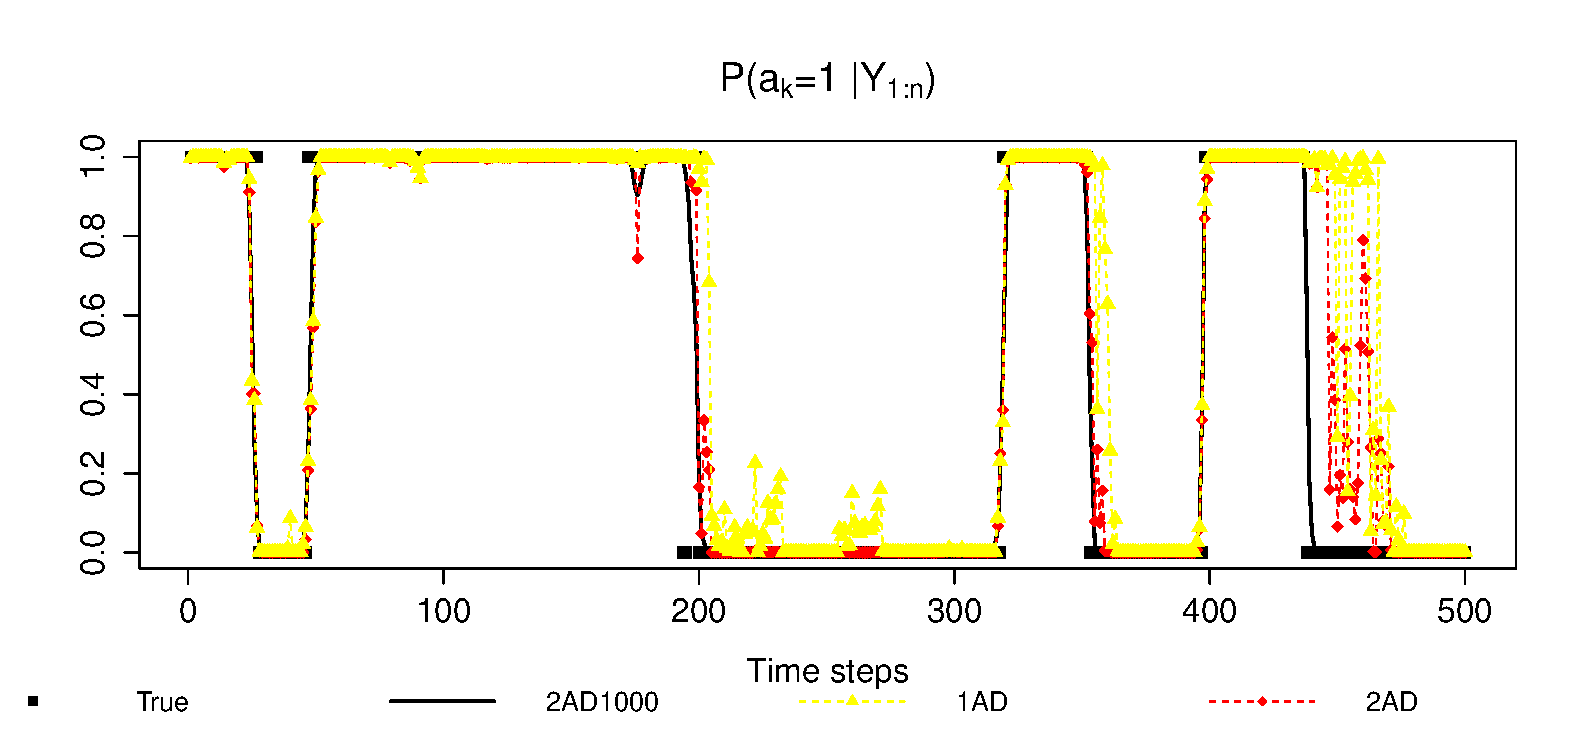
\includegraphics[scale=.5]{Artificial_Compare_Exp1_1_500.eps}
%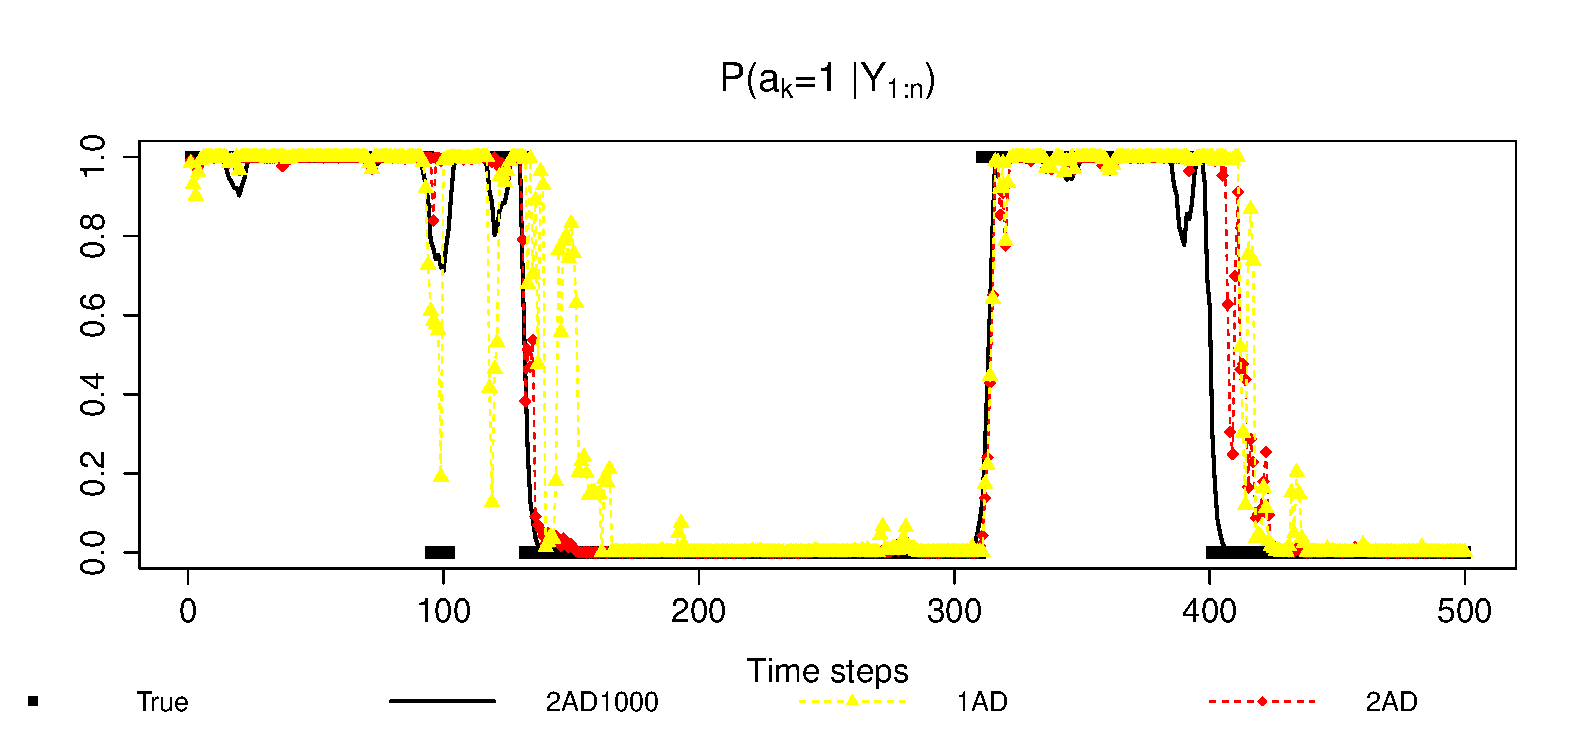
\includegraphics[scale=.5]{Artificial_Compare_Exp2_1_500.eps}
%\caption{estimated probabilities by RBTF in experiment 1 [top] and experiment 2 [bottom] with the two artificial laws: yellow (the first one) and red (the third one).}
%\label{fig:exp:artificial}
%\end{figure}

Figures~\ref{fig:exp1:label} and~\ref{fig:exp2:label} displays the approximations of the  posterior distributions of the labels given by the algorithms using:
\[
\gamma^{}_i (a_i, z_i) = \sum_{k=1}^{N} Q(a^{k}_{i-1},a_i) \omega^{k}_{i-1} \exp\left\{ -\frac{1}{2} \log \left|\barH_{a^k_{i-1}} \right| -\frac{1}{2}\normMat{\barH_{a^k_{i-1}}}{z_i - d_{a^k_{i-1}} -T \mu^k_{i-1} }^2\right\} \eqsp.
\]
In both cases, RBTF behaves slightly better than \cite{briers:doucet:maskell:2010} which does not detect some regime switchings (for instance  at time 780 in Figure~\ref{fig:exp1:label} and at time 300 in Figure~\ref{fig:exp2:label}) or gives false detections (for instance at time 10 in Figure~\ref{fig:exp2:label}).

\begin{figure}
\centering
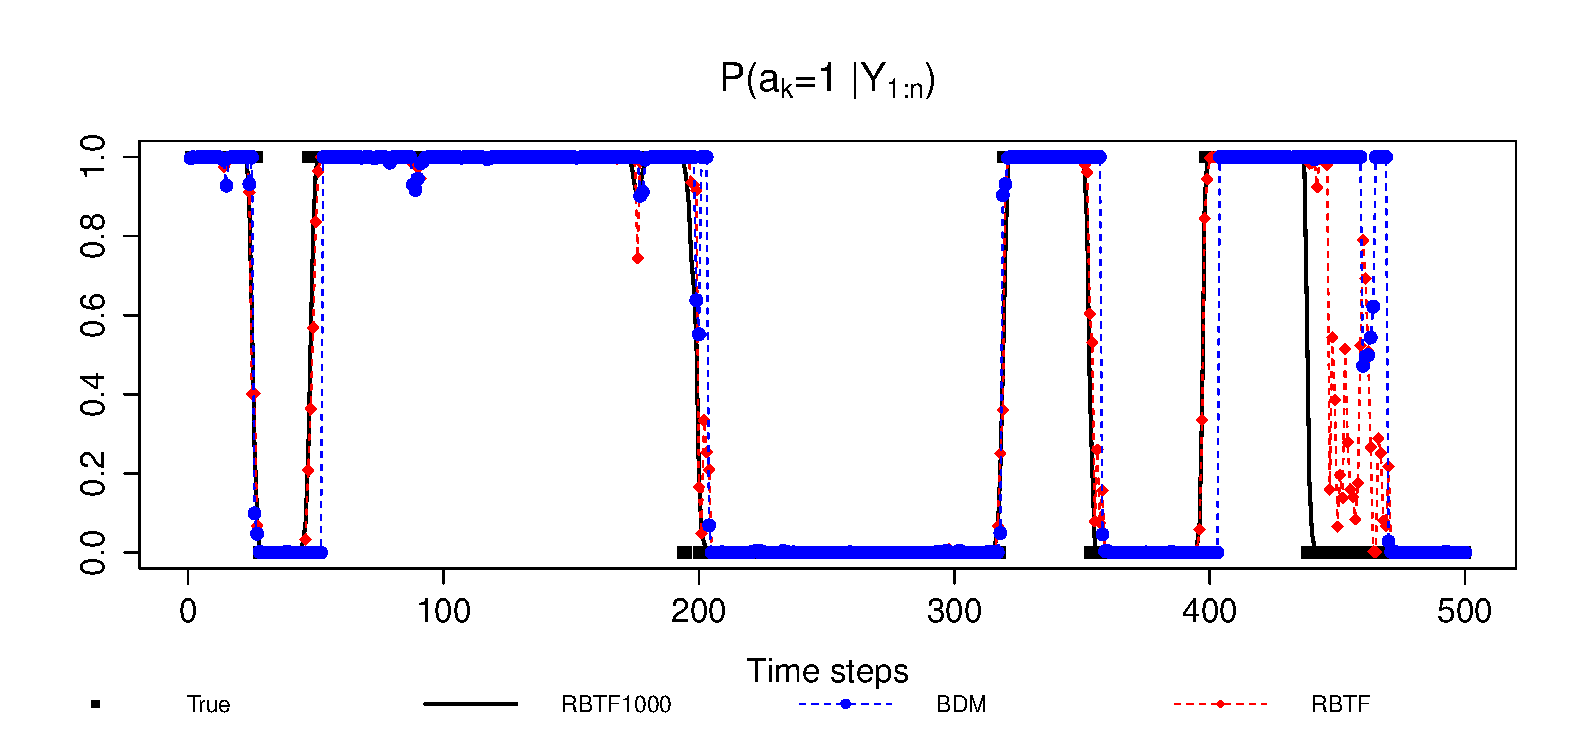
\includegraphics[scale=.5]{N10_1_500.eps}
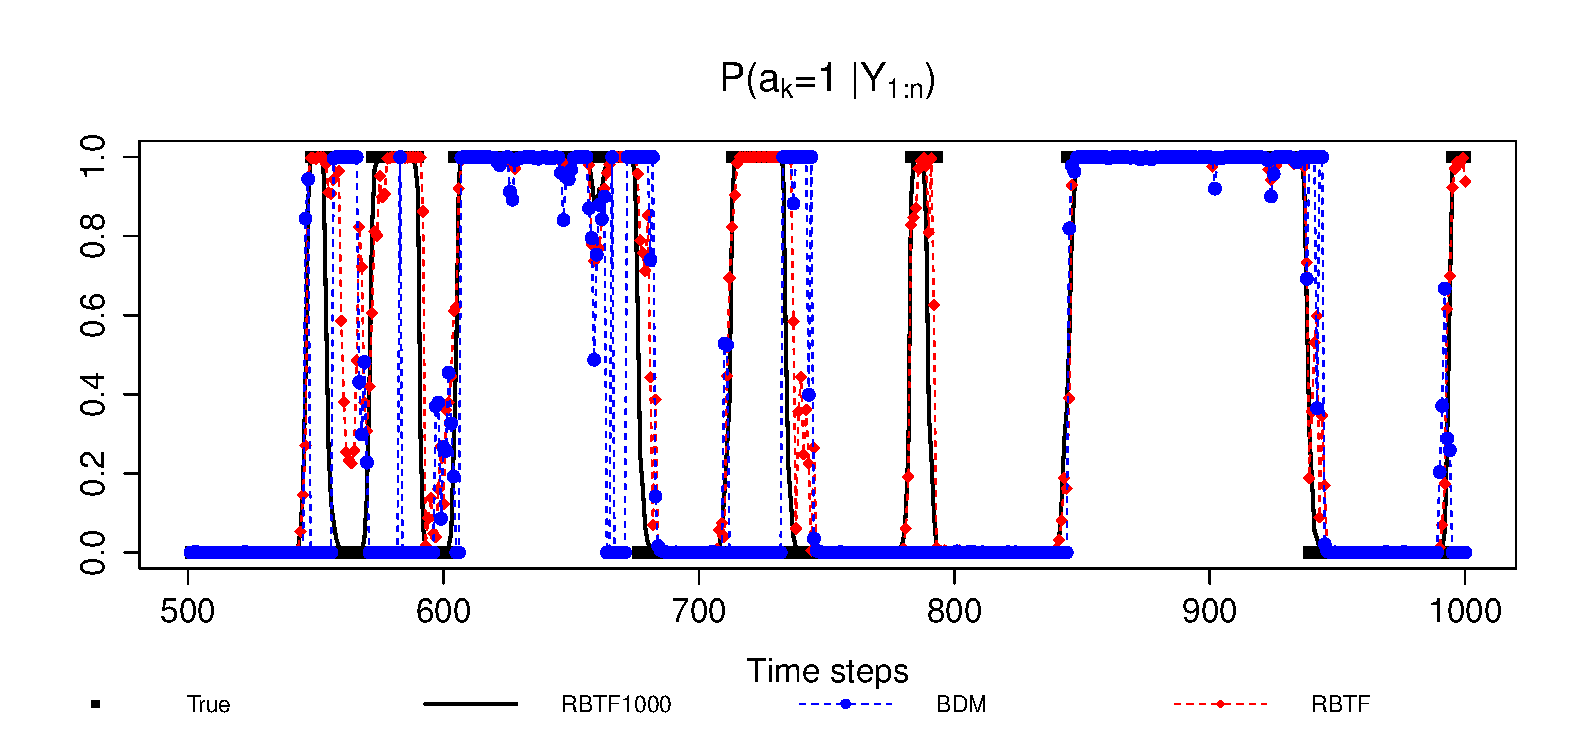
\includegraphics[scale=.5]{N10_501_1000.eps}
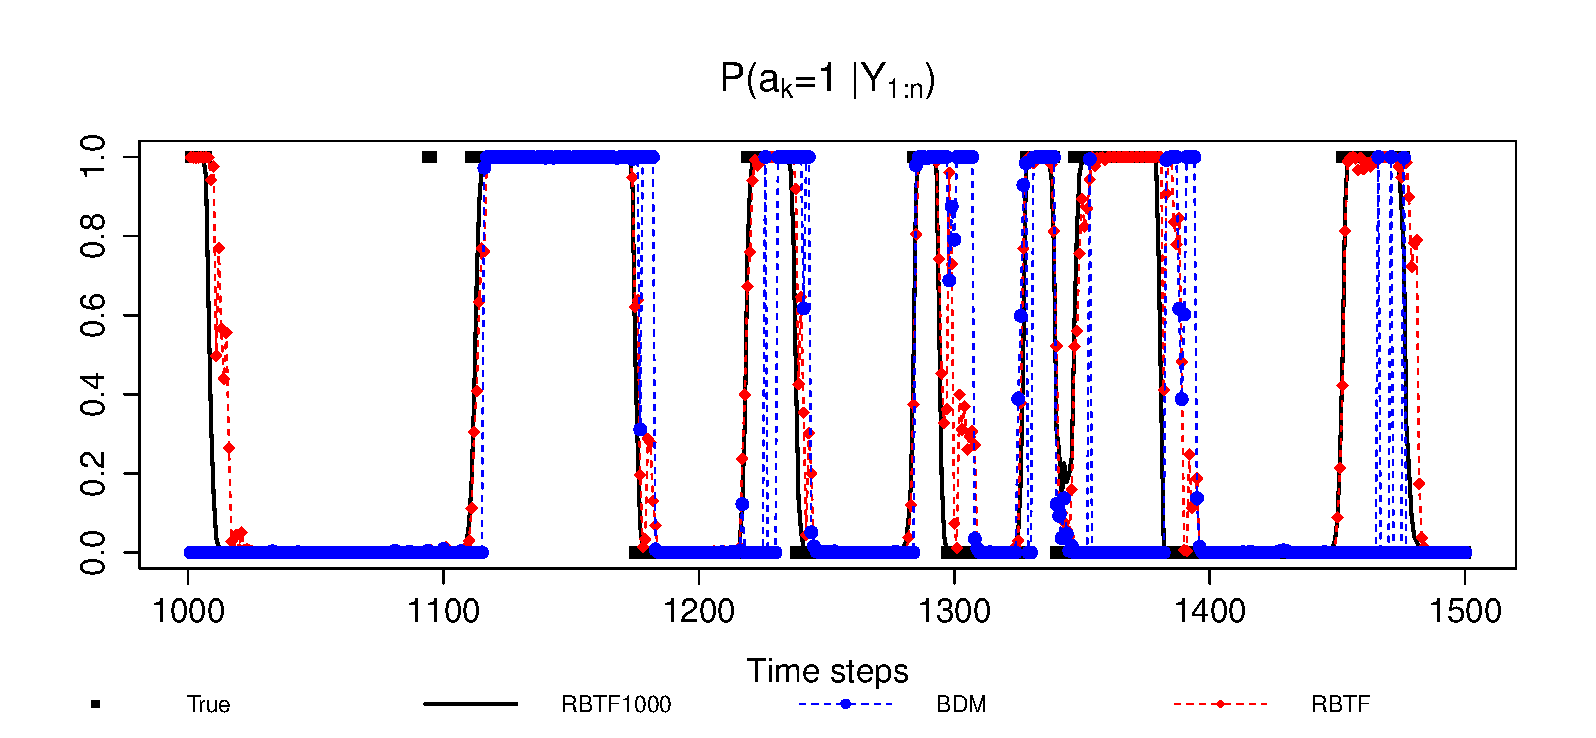
\includegraphics[scale=.5]{N10_1001_1500.eps}
\caption{Experiment 1 - estimated probabilities by \cite{briers:doucet:maskell:2010} (blue) and RBTF (red) with $N=10$ particles,  RBTF with $N=1000$ particles (black line) and true labels (squared black).}
\label{fig:exp1:label}
\end{figure}

\begin{figure}
\centering
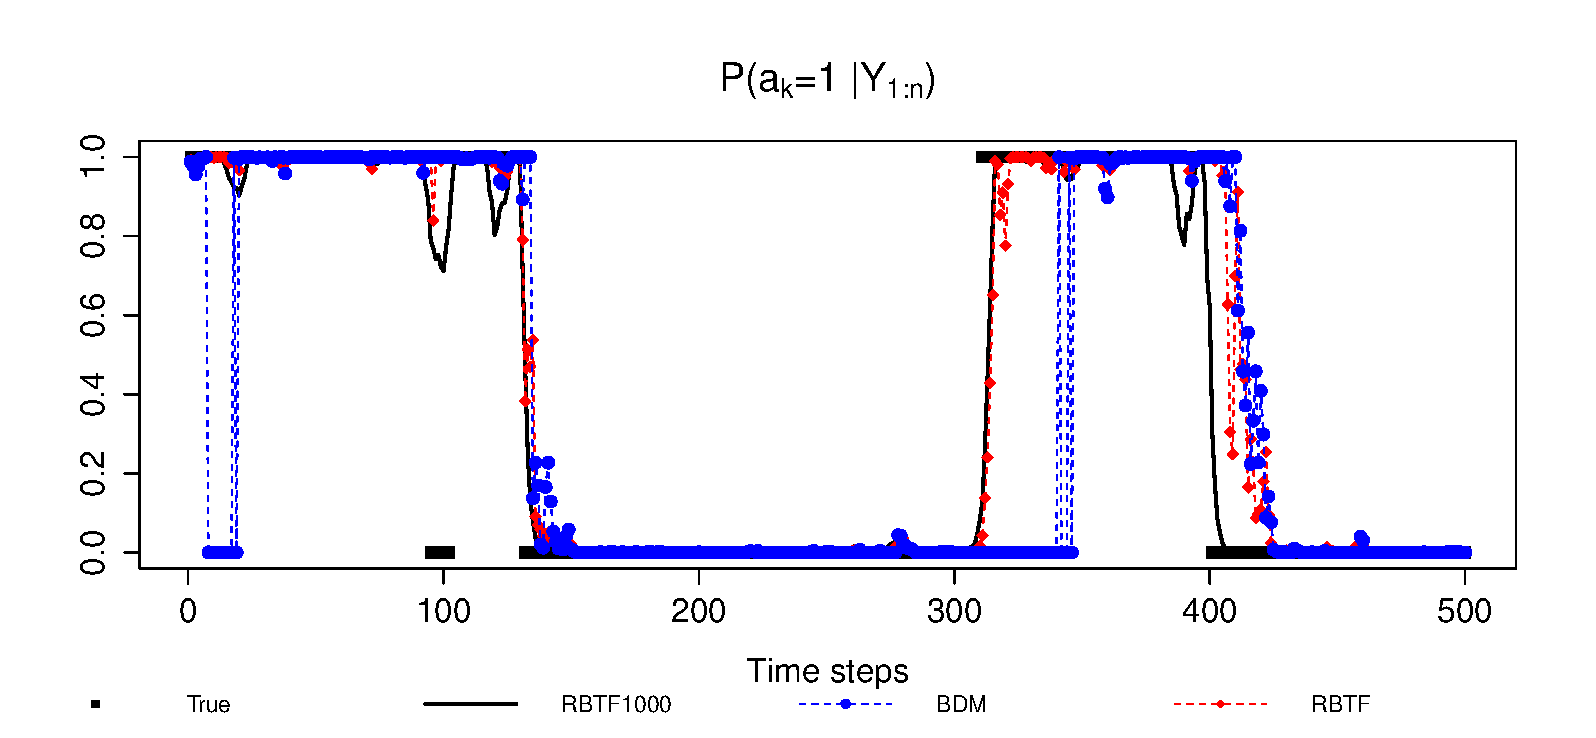
\includegraphics[scale=.5]{N15_1_500.eps}
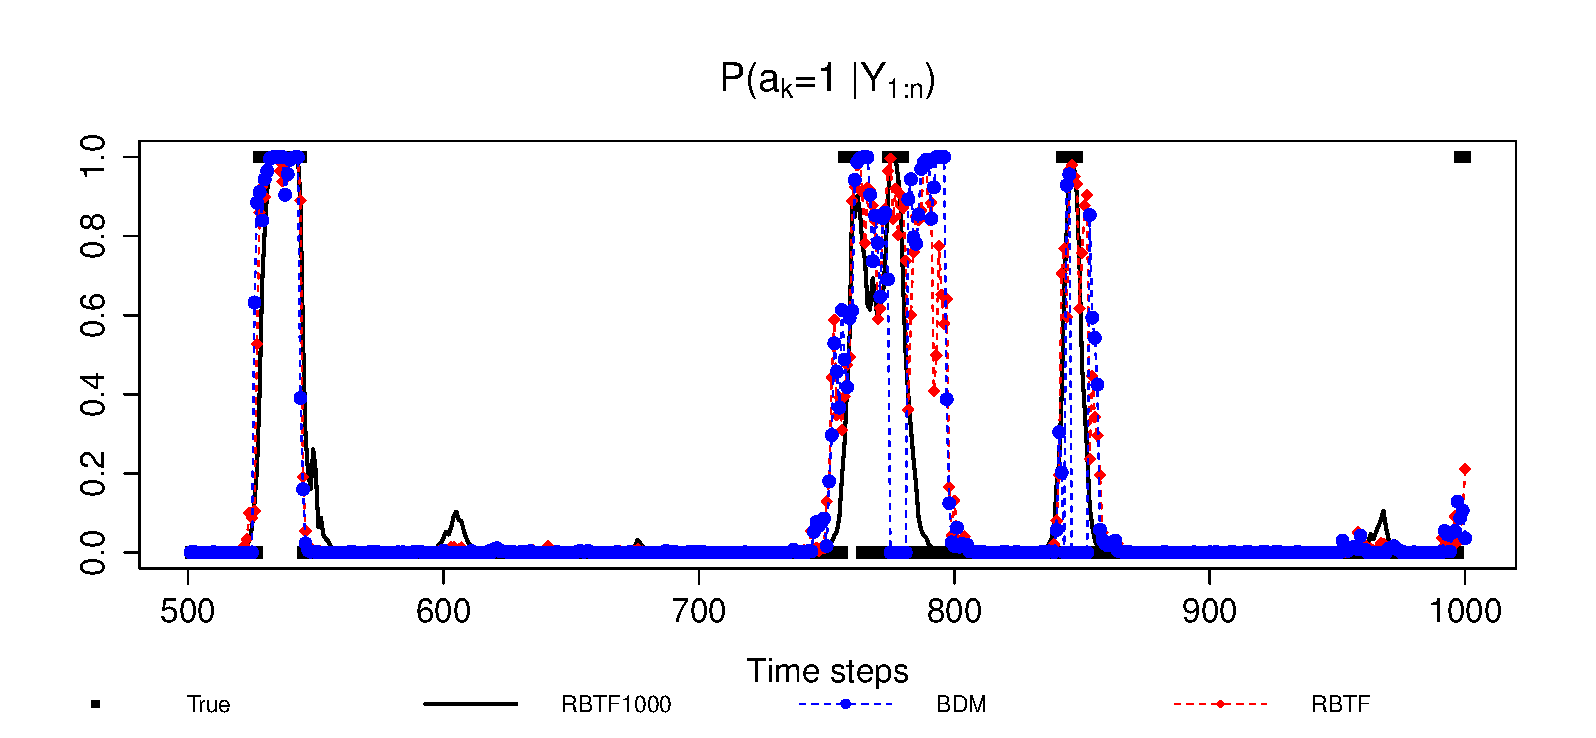
\includegraphics[scale=.5]{N15_501_1000.eps}
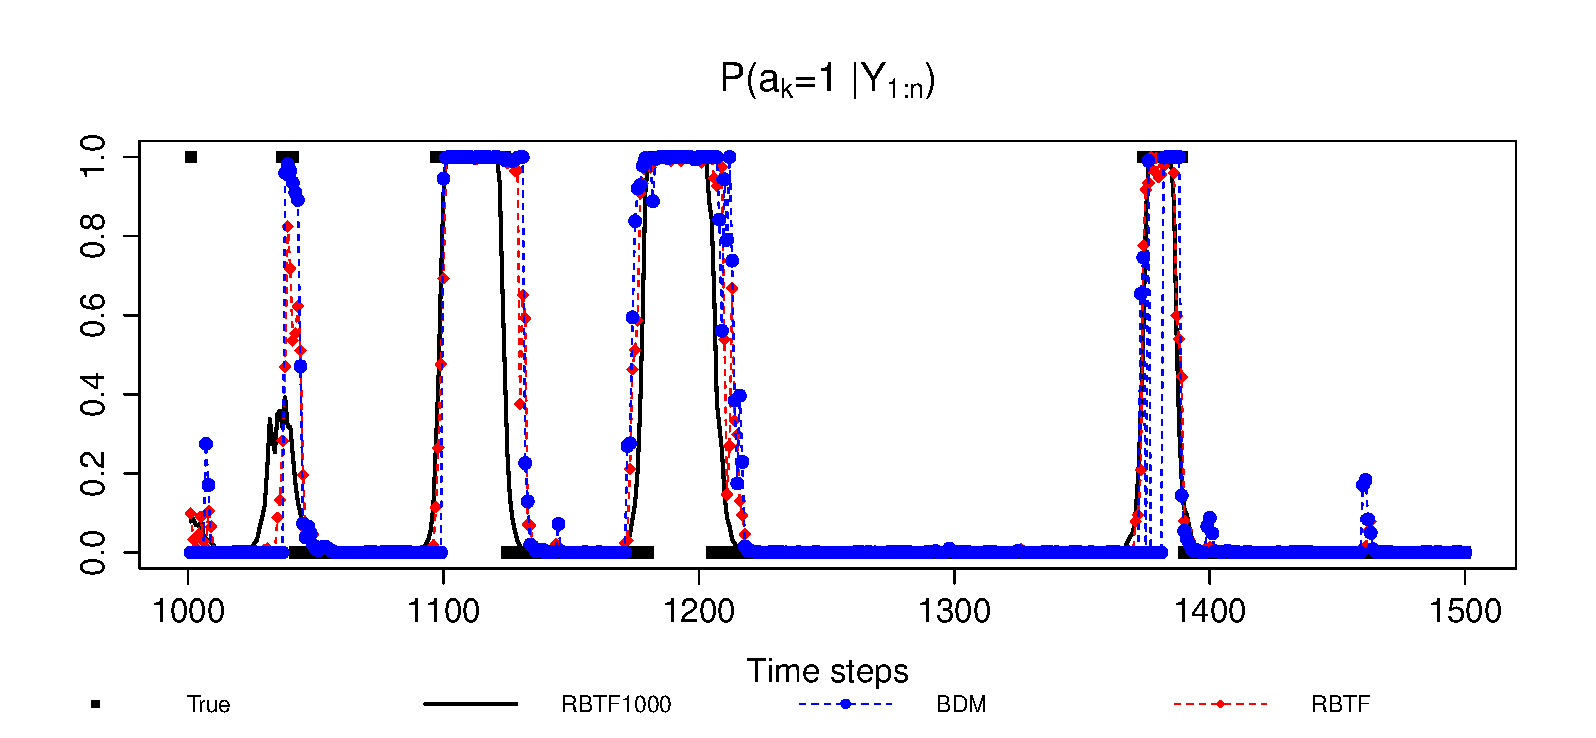
\includegraphics[scale=.5]{N15_1001_1500.eps}
\caption{Experiment 2 - estimated probabilites by \cite{briers:doucet:maskell:2010} (blue) and RBTF (red) with $N=15$ particles, RBTF with $N=1000$ particles (black line) and true labels (squared black).}
\label{fig:exp2:label}
\end{figure}

\subsection{Application to CME crude oil (WTI)}
\label{sec:exp}

\subsubsection*{State dynamics}
Modeling commodity prices is a crucial step to valuate contingent claims related to energy markets and to optimize storage or extraction strategies. In \cite{gibson:schwartz:1990,schwartz:1997}, the authors proposed a model where the spot price of a commodity$(S_t, t \geq 0)$ depends on a second factor $(\delta_t, t \geq 0)$, referred to as the instantaneous convenience yield. This factor plays the role of dividends in equity markets and models the benefit of holding the physical commodity or the storage and maintenance costs required to keep the commodity. In this model, this convenience yield is described as an Ornstein-Uhlenbeck process:
\begin{align*}
\rmd S_{t} & = (r-\delta_{t})S_{t}\rmd t+\sigma S_{t} \rmd W_{t}^{1} \eqsp,\\
\rmd \delta_{t} & = \kappa(\alpha-\delta_{t})\rmd t+\eta \rmd W_{t}^{2} \eqsp, \quad \rmd \langle W_t^1, W_t^2\rangle = \rho \rmd t\eqsp,
\end{align*}
where the parameter $\left(r, \sigma, \kappa, \alpha, \eta, \rho \right)$ are constant and $( (W_t^1,W_t^2), t \geq 0)$ are standard Brownian motions. This model appear to be too restrictive as energy markets are not likely to revert to a single equilibrium value. This assumption is relaxed using Markov switching models to allow several possible regimes for the spot price and the convenience yield. Following \cite{almansour:2016}, the spot price and convenience yield are described in this paper as:
\begin{align*}
\rmd S_{t} & = (r-\delta_{t})S_{t}\rmd t+\sigma_{a_t} S_{t}\rmd W_{t}^{1} \eqsp,\\
\rmd\delta_{t} & = \kappa_{a_t}(\alpha_{a_t} -\delta_{t})\rmd t+\eta_{a_t} \rmd W_{t}^{2} \eqsp, \quad \rmd\langle W_t^1, W_t^2\rangle = \rho_{a_t} \rmd t\eqsp,
\end{align*}
where $(a_t)_{t\ge 0}$ is a finite state space Markov process. 
%We assume that $J=2$, each regime characterizing the slope of the future curve. A backwardation regime (resp. contango regime) is defined as a negative slope (resp. a positive slope). 
Statistical estimation is performed using market observations and cannot be done directly under the risk-neutral probability but under the historical probability $\mathbb{P}$. It is assumed that each factor (spot, convenience yield) has its own constant market price of risk, $\lambda^S$ for $S_t$ and $\lambda^{\delta}$ for $\delta_t$. The historical dynamics of the Gibson-Schwartz model is then described as follows:
\begin{align*}
\rmd S_{t} & = (\mu -\delta_{t})S_{t}\rmd t+\sigma_{a_t} S_{t} \rmd \widetilde{W}_{t}^{1} \eqsp,\\
\rmd \delta_{t} & = \kappa_{a_t}(\widetilde{\alpha}_{a_t}-\delta_{t})\rmd t+\eta_{a_t} \rmd \widetilde{W}_{t}^{2} \eqsp, \quad \rmd \langle \widetilde{W}_t^1, \widetilde{W}_t^2\rangle = \rho \rmd t\eqsp,
\end{align*}
where $( (\widetilde{W}_t^1,\widetilde{W}_t^2), t \geq 0)$ are standard Brownian motions under the historical probability $\mathbb{P}$ with  correlation $\rho_{a_t}$, $\mu = r - \lambda^S$ and $\widetilde{\alpha}_{a_t} = \alpha_{a_t} - \lambda^{\delta}/\kappa_{a_t} $. This model allows to exhibit fundamental features of commodity future prices, which typically display different regimes of volatility and/or convenience yield. A two-regime model is already sufficient to produce stylized effects such as contango (increase of future prices) and backwardation (decrease of future prices).  Assuming that the switching rate between regimes is small compared to the inverse of the discretization period, the discretized version of the spot price and convenience yield $Z_i= (\ln S_i, \delta_i)$ (the sampling period is taken to be 1) is modeled as a Conditionally Linear Gaussian Model. The explicit integration of this SDE detailed in Lemma~\ref{lem:integratedSDE} yields the following discrete time model for $(Z_i)_{i\ge 0}$:
\[
Z_i = d_{a_{i-1}} + T_{a_{i-1}} Z_{i-1} + H_{a_{i-1}} \varepsilon_i\eqsp,
\]
%where (setting $\Delta t_i = t_i-t_{i-1}=1$):
%\[
%d_{j} \eqdef
%\begin{pmatrix} \left[r- \alpha_{j} - \sigma^2_{j}/2 \right]  + \alpha_{j}[1-\rme^{-\kappa}]/\kappa\\
%\alpha_{j} [1-\rme^{-\kappa}] \end{pmatrix}\eqsp, \;\; T \eqdef
%\begin{pmatrix} 1 & -[1-\rme^{-\kappa}]/\kappa \\ 0 & \rme^{-\kappa} \end{pmatrix} \eqsp,
%\]
%\begin{align*}
%\barH_{j}(1,1) &= \sigma^2_{j} + \eta^2_{j}\left\{1 + (1-\rme^{-2\kappa})/(2\kappa) - 2(1-\rme^{-\kappa})/\kappa\right\}/\kappa^2
%- 2\rho_{j} \eta_{j} \sigma_{j}\left\{ 1 - (1-\rme^{-\kappa})/\kappa \right\}/\kappa\eqsp, \\
%\barH_{j}(1,2) & = \left(\rho_{j} \eta_{j} \sigma_{j}-\eta^2_{j}/\kappa\right)\left(1-\rme^{-\kappa} \right)/\kappa + \eta^2_{j}\left(1-\rme^{-2\kappa} \right)/(2\kappa^2)\eqsp,\\
%\barH_{j}(2,1) &= \barH_{j}(1,2)\eqsp,\quad \barH_{j}(2,2) = \eta^2_{j}\left( 1-\rme^{-2\kappa} \right)/(2\kappa)\eqsp.
%\end{align*}
where (with $\barH_{a_{i-1}} \eqdef H_{a_{i-1}}H'_{a_{i-1}}$ and $\Delta t_i = t_i-t_{i-1}$):
\begin{align*}
d_{a_{i-1}} &\eqdef
\begin{pmatrix} \left[\mu- \widetilde{\alpha}_{a_{i-1}} - \sigma^2_{a_{i-1}}/2 \right] \Delta t_i + \widetilde{\alpha}_{a_{i-1}}[1-e^{-\kappa_{a_{i-1}} \Delta t_i}]/\kappa_{a_{i-1}}\\
\widetilde{\alpha}_{a_{i-1}} [1-e^{-\kappa_{a_{i-1}} \Delta t_i}] \end{pmatrix}\eqsp,\\
T_{a_{i-1}} &\eqdef
\begin{pmatrix} 1 & -[1-e^{-\kappa_{a_{i-1}} \Delta t_i}]/\kappa_{a_{i-1}} \\ 0 & e^{-\kappa_{a_{i-1}} \Delta t_i} \end{pmatrix} \eqsp,\\
\barH_{a_{i-1}}(1,1) &= \sigma^2_{a_{i-1}} \Delta t_i + \eta^2_{a_{i-1}}\left\{\Delta t_i + (1-e^{-2\kappa_{a_{i-1}} \Delta t_i})/(2\kappa_{a_{i-1}}) - 2(1-e^{-\kappa \Delta t_i})/\kappa_{a_{i-1}}\right\}/\kappa_{a_{i-1}}^2 \\
&\hspace{5.2cm} - 2\rho_{a_{i-1}} \eta_{a_{i-1}} \sigma_{a_{i-1}}\left\{ \Delta t_i - (1-e^{-\kappa_{a_{i-1}} \Delta t_i})/\kappa_{a_{i-1}} \right\}/\kappa\eqsp, \\
\barH_{a_{i-1}}(1,2) & = \left(\rho_{a_{i-1}} \eta_{a_{i-1}} \sigma_{a_{i-1}}-\eta^2_{a_{i-1}}/\kappa_{a_{i-1}}\right)\left(1-e^{-\kappa_{a_{i-1}}\Delta t_i} \right)/\kappa_{a_{i-1}} \\
&\hspace{5.2cm}+ \eta^2_{a_{i-1}}\left(1-e^{-2\kappa_{a_{i-1}} \Delta t_i} \right)/(2\kappa_{a_{i-1}}^2)\eqsp,\\
\barH_{a_{i-1}}(2,1) &= \barH_{a_{i-1}}(1,2)\eqsp,\\
\barH_{a_{i-1}}(2,2) &= \eta^2_{a_{i-1}}\left( 1-e^{-2\kappa_{a_{i-1}}\Delta t_i} \right)/(2\kappa_{a_{i-1}})\eqsp.
\end{align*}
%Remarks que the equations \eqref{eq:modele} under the pricing measure $\mathbb{Q}$ becomes:
%\begin{equation}
%\begin{cases}
%\rmd S_{t} & = (r -\delta_{t})S_{t}\rmd t+\sigma_{a_t} S_{t}\rmd \widetilde{W}_{t}^{1} \eqsp,\\
%\rmd\delta_{t} & = \left[\kappa(\alpha_{a_t} -\delta_{t}) - \lambda\right]\rmd t+\eta_{a_t} \rmd \widetilde{W}_{t}^{2} \eqsp, \quad \rmd\langle \widetilde{W}_t^1, \widetilde{W}_t^2\rangle = \rho_{a_t} \rmd t\eqsp.
%\end{cases}
%\end{equation}
%where the constant $\lambda$ denotes the market price of convenience yield risk and $\widetilde{W}^1, \widetilde{W}^2$ are two $\mathbb{Q}-$Brownian motions. By introducing a new mean-reversion level for the convenience yeild process under $\mathbb{Q}$ 
%\[
%\widetilde{\alpha} = \alpha - \lambda/\kappa 
%\]
%we obtain the dynamics:
%\[
%\rmd\delta_{t} = \kappa(\widetilde{\alpha}_{a_t} -\delta_{t}) \rmd t+\eta_{a_t} \rmd \widetilde{W}_{t}^{2}
%\]
%The behaviors of $Z_i$ under $\mathbb{Q}$ is $Z_i = \widetilde{d}_{a_{i-1}} + T Z_{i-1} + H_{a_{i-1}} \varepsilon_i 
%$ with 
%\[
%\widetilde{d}_{a_{i-1}} \eqdef
%\begin{pmatrix} \left[r - \widetilde{\alpha}_{a_{i-1}} - \sigma^2_{a_{i-1}}/2 \right] \Delta t_i + \widetilde{\alpha}_{a_{i-1}}[1-e^{-\kappa \Delta t_i}]/\kappa\\
%\widetilde{\alpha}_{a_{i-1}} [1-e^{-\kappa \Delta t_i}] \end{pmatrix}\eqsp,
%\]
%The transition matrix $Q$ is assumed to be the same under the pricing measure. 
\subsubsection*{Observation model}
The observations are Wednesday future contracts of the West Texas Intermediate crude oil (WTI) traded in the Chicago Mercantile Exchange (CME) from $11$ January 1995 to $13$ November 2013. The contracts are numbered $F_1, F_2, \ldots, F_{36}$ where $F_1$ (or front month) is the earliest delivery future contract, $F_2$ is the second earliest delivery future contract and so on. Among these $36$ contracts, the four future contracts: $F_1, F_4, F_6, F_{13}$ are used since their trading volumes and their impacts on the Term Structures are the most important ($F_1$ is the most liquid contract, $F_{13}$ characterizes the gap between prices over a one year period, $F_4$ and $F_6$ are intermediate future contracts that are mostly traded). As in \cite{almansour:2016}, we consider that each  future contract has a fixed time to maturity: $F_1, F_4, F_6, F_{13}$ have time to  maturity $4$, $16$, $26$, $56$ weeks.  Our time series contains $n =975$ weekly data with $534$ in backwardation and $441$ in contango (the backwardation effect is more frequent with crude oil data). At each time $t_i = i\Delta t$, with $\Delta t = 0.0192$, the observations of the $\dimy = 4$ future prices are $Y_i \eqdef (\ln(F^{(market)}_{i\Delta t,m_1}), \ldots, \ln(F^{(market)}_{i\Delta t,m_{\dimy}}))'$, where $F_{t_i,m}$ is the future price at $t_i$ for a maturity  $m$ weeks.
%In addition, the backwardation is more likely to stay in backwardation than switch to contango and the same holds for the contango regime.

\medskip
 
Following \cite{almansour:2016}, it is assumed that $\kappa_1 = \kappa_2 = \kappa$ (and therefore $T_1=T_2=T$) to obtain a closed form solution for $F_{t_i,m}$ which may be written: 
\[
F_{t_i,m} \eqdef \exp\left( \mathsf{A}_{m}(a_{i}) + \mathsf{B}_{m} Z_{i}\right)\eqsp,
\]
where $\mathsf{B}_0	= \begin{pmatrix}1 & 0 \end{pmatrix}$ and  $\mathsf{B}_m    = \mathsf{B}_{m-1} T$ so that  $ \mathsf{B}_m= \begin{pmatrix} 1 & -\left(1-\rme^{-\kappa m \Delta t}\right)/\kappa \end{pmatrix}$ and
%$B_\tau$ is the $1 \times 2$ matrix given by $B_{\tau} \eqdef  \begin{pmatrix} 1 &  -(1-e^{-\kappa \tau})/\kappa \end{pmatrix}$ and
%for all $1\le j\le J$, $A_0(j) \eqdef 0$. Define $F_{i,m} \eqdef F_{i\Delta t, m \Delta t }$ and $\mathcal{F}_i$ the $\sigma$-field generated by $(a_k)_{0\le k \le i}$ and $(Z_k)_{0\le k \le i}$. By definition of future prices and the assumption that there is no regime switching between $t_i$ and $t_{i+1}$, we have:
%%\begin{align*}
%%A_{t,\tau} &\eqdef r \tau - \int^{\tau}_0 \alpha_{a_{t+s}} \left(1- e^{-\kappa(\tau-s)} \right)\rmd s + (1/\kappa^2)\int^{\tau}_0 \eta^2_{a_{t+s}} \left(1-e^{-\kappa (\tau-s)}\right)^2 \rmd s \\
%%&\hspace{7cm}  - (2/\kappa)\int^{\tau}_0 \rho_{a_{t+s}} \eta_{a_{t+s}}\sigma_{a_{t+s}} \left( 1 -e^{-\kappa \left(\tau-s\right)} \right)\rmd s \eqsp,\\
%%B_{\tau} &\eqdef  \begin{pmatrix} 1 &  -(1-e^{-\kappa \tau})/\kappa \end{pmatrix}\eqsp.
%%\end{align*}
%\begin{align*}
%F_{i,m} &= \exp (A_m(a_i) + B_m Z_i)\eqsp,\\
%&=\mathbb{E}\left[\exp (A_{m-1}(a_{i+1}) + B_{m-1} Z_{i+1})\middle|\mathcal{F}_i\right]\eqsp,\\
%&= \mathbb{E}\left[\sum^J_{k=1} 1_{a_{i+1}=k}\exp (A_{m-1}(k) + B_{m-1} Z_{i+1})\middle|\mathcal{F}_i\right] \eqsp,\\
%&= \mathbb{E}\left[\sum^J_{k=1} 1_{a_{i+1}=k}\exp \left(A_{m-1}(k) + B_{m-1} ( d_{a_i} + T Z_i + H_{a_i} \epsilon_{i+1} ) \right)\middle|\mathcal{F}_i\right] \eqsp,\\
%&= \sum^J_{k=1} q(a_i,k) \exp \left(A_{m-1}(k) + B_{m-1} d_{a_i} + B_{m-1} \barH_{a_i} B'_{m-1}/2 + B_{m-1} T Z_i \right)\eqsp.
%\end{align*}
%From the above equality, we obtain,
for all $1\le j\le J$, $\mathsf{A}_0(j) = 0$,  and
\begin{equation*}
\mathsf{A}_m(j) = \ln \left(\sum^J_{k=1} Q(j,k) \exp(\mathsf{A}_{m-1}(k)) \right) + \mathsf{B}_{m-1} d_j + \frac{1}{2} \mathsf{B}_{m-1} \barH_j B'_{m-1}\eqsp.
\end{equation*}
Therefore, the observations of the  logfuture prices are given, for all $1\le i\le n$, by: 
\[
Y_i = c_{a_i} + B Z_i + G \eta_i\eqsp,
\] 
where $\xi_i$ is a standard multivariate Gaussian random variable and:
\[
c_{j}' = \begin{pmatrix} \mathsf{A}_{m_1}(j) & \ldots & \mathsf{A}_{m_{\dimy}}(j) \end{pmatrix}\eqsp,
\;\;\;
B' = \begin{pmatrix}\mathsf{B}_{m_1}' &  \ldots & \mathsf{B}_{m_{\dimy}}' \end{pmatrix}\eqsp, \;\;\;
G = \mathrm{diag}(g_1, \ldots , g_{d} )\eqsp.
\]
The model is then driven by the parameter:
\[
\theta \eqdef \{\pi, Q, \mu_1, \Sigma_1, \kappa, (\alpha_j)_{1\leq j\leq J}, (\sigma_j)_{1\leq j\leq J}, (\eta_j)_{1\leq j\leq J}, (\rho_j)_{1\leq j\leq J}, \mu, (\lambda_j)_{1\leq j\leq J}, (g_{\ell})_{1\leq \ell\leq d} \}\eqsp.
\]
The aim of this section is to estimate $\theta$ and the posterior probabilities $\mathbb{P}(a_k=j|Y_{1:n})$, $1\le k \le n$, $1\le j \le J$. Given the observations $Y_{1:n}$, the EM algorithm introduced in \cite{dempster:laird:rubin:1977} maximizes the incomplete data log-likelihood $\theta\mapsto \ell_{\theta}^{n}$ defined by
\begin{equation*}
%\label{eq:loglik}
\ell_{\theta}^{n}(Y_{1:n}) \eqdef \log\left(\sum_{a_1=1}^J\ldots\sum_{a_n=1}^J\int p_{\theta}(a_{1:n},z_{1:n},Y_{1:n})\,\rmd z_{1:n}\right)\eqsp,
\end{equation*}
where the complete data likelihood $p_{\theta}$ is given by
\begin{equation*}
%\label{eq:completelik}
p_{\theta}(a_{1:n},z_{1:n},Y_{1:n}) \eqdef \pi(a_1)\phi_{\mu_1,\Sigma_1}(z_1)g_{\theta}(a_1,z_1;Y_1)\prod^{n}_{i=2}Q(a_{i-1},a_i)m_{\theta}\left(a_{i},z_{i-1};z_i\right)g_{\theta}(a_i,,z_i;Y_i)\eqsp,
\end{equation*}
where $\phi_{\mu_1,\Sigma_1}$ is the Gaussian probability density function with mean $\mu_1$ and variance $\Sigma_1$.
Denote by $\mathbb{E}_{\theta}\left[\cdot\middle|Y_{1:n}\right]$  the conditional expectation given $Y_{1:n}$ when the parameter value is $\theta$. The EM algorithm iteratively builds a sequence $\{\theta_{p}\}_{p\ge 0}$ of parameter estimates following the two steps:
\begin{enumerate}%[label=\roman*)]
	\item {\bf E-step}: compute $\theta \mapsto Q(\theta,\theta_{p})\eqdef \mathbb{E}_{\theta_p}\left[\log p_{\theta}(X_{1:n},Y_{1:n})\middle|Y_{1:n}\right]$ ;
	\item {\bf M-step}: choose $\theta_{p+1}$ as a maximizer of $\theta \mapsto Q(\theta,\theta_{p})$.
\end{enumerate}
%\paragraph{E-step}
%By \eqref{eq:completelik}, the intermediate quantity $Q(\theta,\theta_p)$ may be written (up to some additive constant which does not depend on $\theta$) $Q(\theta,\theta_p) = I^{n}_{1,\theta_p} + J^{n}_{1,\theta_p} + \sum_{i=2}^nI^{n}_{i,\theta_p} + \sum_{i=2}^nJ^{n}_{i,\theta_p}$,
%where
%\begin{align*}
% I^{n}_{1,\theta_p} &\eqdef \mathbb{E}_{\theta_p}\left[\log\phi_{\mu_1,\Sigma_1}(Z_1)\middle|Y_{1:n}\right]\eqsp,\\
% &= - \frac{1}{2}\log|\Sigma_1| -\frac{1}{2}\mathrm{Tr}\left(\Sigma_1^{-1}\mathbb{E}_{\theta_p}\left[Z_1Z'_1\middle|Y_{1:n}\right]\right) +\mu'_1\Sigma_1^{-1}\mathbb{E}_{\theta_p}\left[Z_1\middle|Y_{1:n}\right]- \frac{1}{2}\mu'_1\Sigma_1^{-1}\mu_1\eqsp,\\
% J^{n}_{1,\theta_p} &\eqdef \mathbb{E}_{\theta_p}\left[\log g_{\theta}(a_1,z_1;Y_1)\middle|Y_{1:n}\right]\eqsp,\\
% &= -\frac{1}{2}\log|\barG|-\frac{1}{2}\sum_{j=1}^J\mathrm{Tr}\left(\barG^{-1}\mathbb{E}_{\theta_p}\left[\left(Y_1-c_{j}-BZ_1\right)\left(Y_1-c_{j}-BZ_1\right)'\1_{a_1=j}\middle|Y_{1:n}\right]\right)
%\end{align*}
%and, for all $2\le i\le n$,
%\begin{align*}
% I^{n}_{i,\theta_p} &\eqdef\mathbb{E}_{\theta_p}\left[\log m_{\theta}\left(a_{i-1},z_{i-1};z_i\right)\middle|Y_{1:n}\right]\eqsp,\\
% &= -\frac{1}{2}\sum_{j=1}^J\log |\barH_{j}|\mathbb{E}_{\theta_p}\left[\1_{a_{i-1}=j}\middle|Y_{1:n}\right]\\
% &\hspace{.4cm}-\frac{1}{2}\sum_{j=1}^J \mathrm{Tr}\left(\barH^{-1}_j\mathbb{E}_{\theta_p}\left[\left(Z_i-d_{j}-TZ_{i-1}\right)\left(Z_i-d_{j}-TZ_{i-1}\right)'\1_{a_{i-1}=j}\middle|Y_{1:n}\right]\right)\eqsp.
% \end{align*}
% \begin{align*}
% J^{n}_{i,\theta_p} &\eqdef\mathbb{E}_{\theta_p}\left[\log g_{\theta}(a_i,z_i;Y_i)\middle|Y_{1:n}\right]\eqsp,\\
% &= -\frac{1}{2}\log|\barG|-\frac{1}{2}\sum_{j=1}^J\mathrm{Tr}\left(\barG^{-1}\mathbb{E}_{\theta_p}\left[\left(Y_i-c_{j}-BZ_i\right)\left(Y_i-c_{j}-BZ_i\right)'\1_{a_i=j}\middle|Y_{1:n}\right]\right)\eqsp.
%\end{align*}
All the conditional expectations involved in $Q(\theta,\theta_p)$ are approximated using our RBTF algorithm to define the SMC approximation  $\theta\mapsto Q^N(\theta,\theta_p)$ of $\theta\mapsto Q(\theta,\theta_p)$.
%\paragraph{M-step}
As the function $\theta\mapsto Q^N(\theta,\theta_p)$ cannot be maximized analytically, the M-step is performed numerically using the Covariance Matrix Adaptation Evolution Strategy (CMA-ES) introduced in \cite{hansen:ostermeier:2001}. This derivative-free optimization procedure is known to perform well in complex multimodal optimization settings, see e.g. \cite{hansen:kern:2004}. 

%In details, among $510$ backwardation there are $485$ data whose regime staying in this regime, the same remarks on $417$ among $441$ contango doesn't change its regime.

%The future expiration date usually expires on the third business day prior to the $25-th$ calendar day of the month preceeding the delivery month
%\footnotetext{For WTI crude oil, trading in the current delivery month shall cease on the third business day prior to the $25$th calendar day of the month preceding the delivery month. If the $25$th calendar day of the month is a non-business day, trading shall cease on the third business dat prior to the last business day preceding the $25$th calendar day. See http://www.cmegroup.com for more details}

%Contrary to \cite{almansour:2014}, we calculate the exact time to maturity for each day and each future contract. For example, on $19-05-2010$ the time to maturity of the front contract $F_1$ is only $1$ day (the earliest expiration date is $20-05-2010$) but it is considered with a time to maturity $1$ month in \cite{almansour:2014}. Our calculus takes into account exactly the real time to maturity.

\subsubsection*{Numerical results}
\label{sec:crudeoil}
%Following \cite{carmona:ludkovski:2004}, under the risk neutral probability $\mathbb{Q}$, we assume that the spot price $S_t$ of the Chicago Mercantile Exchange (CME) crude oil and its associated convenience yield $\delta_t$ are solutions to the SDE:
%\begin{align*}
%\rmd S_t &= \left(\tilde{\mu}_{a_{t}} - \delta_t\right) S_t \rmd t + \sigma_{a_t} S_t \rmd \tilde{W}^1_t \eqsp,\\
%\rmd \delta_t &= \kappa \left( \tilde{\alpha}_{a_t} - \delta_t \right) \rmd t + \eta_{a_t} \rmd \tilde{W}^2_t \eqsp,
%\end{align*}
%where $\tilde{W}^1$ and $\tilde{W}^2$ are two correlated Brownian motions under the historical probability $\mathbb{P}$.
%
%In this case,  $\delta_t$ is an Orstein-Uhlenbeck process.
%
%Under the risk-neutral probability $\mathbb{Q}$, this dynamic becomes:
%\begin{align*}
%\rmd S_t &= \left(r - \delta_t\right)S_t \rmd t + \sigma_{a_t} S_t \rmd W^1_t \eqsp,\\
%\rmd \delta_t &= \left[\kappa \left(\alpha_{a_t} - \delta_t \right) - \lambda_{a_t} \right] \rmd t + \eta_{a_t} \rmd  W^2_t \eqsp,
%\end{align*}
%Define $\alpha_{a_t} \eqdef \tilde{\alpha}_{a_t} - \lambda_{a_t}/\kappa$. Therefore, the dynamic of $Z_t = (\ln(S_t), \delta_t)$ under the risk-neutral mesure is:
%\begin{align*}
%\rmd \ln(S_t) &= \left(r - \delta_t- \sigma^2_{a_t}/2 \right) dt + \sigma_{a_t} \rmd W^1_t \eqsp,\\
%\rmd \delta_t &= \kappa\left( \alpha_{a_t} - \delta_t\right)dt + \eta_{a_t} \rmd W^2_t \eqsp,
%\end{align*}
%where $(a_t)_{t\ge 0}$ is a Markov process taking values in  $\{1,\ldots,J\}$ indicating the market regime and $W^1$ and $W^2$ are Brownian motions under $\mathbb{Q}$ such that $\rmd<W^1, W^2>_t = \rho_{a_t}\rmd t$. The interest rate $r$ is constant and $\lambda_{a_t}$ is a risk associated with the convenience yield dynamic when the market regime is $a_t$. In the following, it is assumed that between two consecutive observations at times $t_{i-1}$ and $t_{i}$, the market regime is fixed so that the solutions to the previous SDE may be computed explicitly if $a_t$ is set to $a_{i-1} = a_{t_{i-1}}$. Therefore, it is assumed that the regime indicators are given at times $(t_i)_{i\ge 1}$ by a discrete time Markov chain $(a_{i})_{i\ge 1}$ and do not change between $t_{i-1}$ and $t_{i}$.
%The explicit integration of \eqref{eq:modele} between $t_{i-1}$ and $t_i$ under the approximation that there is no regime change between these two successive time instants provides the following values of the parameter of the discrete time model:
%for $Z_i \eqdef (\ln (S_{t_i}),\delta_{t_i})$:
%\[
%Z_i = d_{a_{i-1}} + T Z_{i-1} + H_{a_{i-1}} \varepsilon_i\eqsp,
%\]
%with $\varepsilon_i$ a standard $2$-dimensional Gaussian random variable and parameters defined as






%For WTI crude oil, trading in the current delivery month shall cease on the third business day prior to the $25$th calendar day of the month preceding the delivery month. If the $25$th calendar day of the month is a non-business day, trading shall cease on the third business dat prior to the last business day preceding the $25$th calendar day. In the event that the official exchange holiday schedule changes subsequent to the listing of a crude oil futures, the originally listed expiration date shall remain in effect. In the event that the originally listed expiration day is declared a holiday, expiration will move to the business day immediately prior. For example, the $25$th Jan $2014$ is sunday, the business day immediately prior is $23$th Jan (friday) to which the $3$rd business day prior is $20th Jan$. Therefore the maturity dates of $Feb 2014$ Contract is $20th Jan 2014$.
%For the CME WTI crude oil, the future prices are informed each trading day for each contract. Based on the expiration date, we may obtain an exact time to maturity for these futures. In our case, we are only interested in certain constant times to maturity: $4W$, $3M$, $6M$, $1Y$, $1,5Y$, $2Y$ and $3Y$. We chose the corresponding future contracts numbers: $1, 3, 7, 13, 19, 25$ and $37$ since this series is near the series $4W, 3M, 6M, 1Y, 1,5Y, 2Y, 3Y$. Futures prices for such fixed time to maturity may be estimated from the existing futures by smoothing splines or linear interpolation method.  For our weekly (every Wednesday) future prices data, we used the linear interpolation from $1995$-$01$-$01$ to $2013$-$05$-$01$. The period $1995$-$01$-$01$ to $2013$-$05$-$01$ used for CME WTI Crude Oil future prices is the same as the one for the data used in \cite{almansour:2014} so that we may use the same weekly transition matrix $Q$: $Q(1,1) = 0.9807$ and $Q(2,2) = 0.9734$ (the authors used the New York Mercantile Exchange (NYMEX) WTI crude oil). The initials values for the EM algorithm are given below:

The initial transition probability in CMA-ES is chosen as $Q(1,1) = 0.98, \; Q(2,2) = 0.97$ and $\pi(1) = \pi(2) = 0.5$ where the number $1$ represents the backwardation regime and $2$ represents the contango regime. The other parameters are initialized as shown in the following table:
\begin{figure}[h!]
	\centering
	\begin{tabular}{||c|c|c|c|c|c|c|c|c|c|c|c|c|c|c|c||}
		$\kappa$ & $\alpha_1$ & $\alpha_2$ & $\sigma_1$ & $\sigma_2$ & $\eta_1$ & $\eta_2$ & $\rho_1$ & $\rho_2$ & $\mu$ & $\lambda_1$ & $\lambda_2$ & $g_1$ & $g_2$ & $g_3$ & $g_4$ \\
		\hline
		5.0 & 0.1 & -0.05 & 0.4 & 0.4 & 0.5 & 0.5 & 0.75 & 0.65 & 0.0 & 0.0 & 0.0 & 0.1 & 0.1 & 0.1 & 0.1
	\end{tabular}
	\caption{Initial values for the EM algorithm.}
\end{figure}\\
The number of particles is set to $N = 100$, $\Delta t = 1/52$. % and the backward filter is based on the  third artificial distribution introduced in Section~\ref{sec:artificial:distribution}. 
The interest rate is $r = 0.0296$ as in \cite{almansour:2016}. The initial guess for the mean and variance of the initial state are
\[
\mu_1 = \begin{pmatrix} \ln F^{(market)}_{1,4} & r-\cfrac{\ln F^{(market)}_{1,16}-\ln F^{(market)}_{1,4}}{(16-4)\Delta t} \end{pmatrix}\quad \mbox{and}\quad \Sigma_1 = \begin{pmatrix} 0.05 & 0 \\ 0 & 0.05 \end{pmatrix}\eqsp.
\]
The CMA-ES algorithm is used with an initial standard deviation for the parameters $\sigma_{cmaes} = 0.005$, a number of selected search points $\mu_{cmaes} = 20$ and a population size $\lambda_{cmaes} = 100$. The algorithm is stopped after $10000$ iterations.
%and its bounded conditions are \\
%\begin{tabular}{cccccccccccccc}
%PAR & $\kappa$ & $\alpha_1$ & $\alpha_2$ & $\sigma_1$ & $\sigma_2$ & $\eta_1$ & $\eta_2$ & $\rho_1$ & $\rho_2$ & $g_1$ & $g_2$ & $g_3$ & $g_4$ \\
%\hline
%INF & 0.01 & -10.0 & -10.0 & 0.01 & 0.01 & 0.01 & 0.01 & 0.01 & 0.01 & 1e-10 & 1e-10 & 1e-10 & 1e-10 \\
%SUP & 1e10 & 10.0 & 10.0 & 1e10 & 1e10 & 1e10 & 1e10 & 1.0 & 1.0 & 1.0 & 1.0 & 1.0 & 1.0 \\
%\end{tabular}
In Gibson-Schwartz model \cite{gibson:schwartz:1990}, a stronger backwardation effect implies a greater value for $\alpha$ for the same values of the other parameters. For the CME WTI Crude Oil, backwardation effect is more frequent than contango effect so that $\alpha_1$ should be greater than $\alpha_2$. Therefore, this condition is imposed for all simulations in the CMA-ES algorithm. The results after $2500$ iterations of the EM algorithm are given in Figure~\ref{fig:CMEfinalestimates}.
\begin{table}[h!]
	\centering
	\begin{tabular}{||c|c|c|c|c|c|c|c|c|c|c||c|clc|c|c||}
		Parameter&$\kappa$ & $\alpha_1$ & $\alpha_2$ & $\sigma_1$ & $\sigma_2$ & $\eta_1$ & $\eta_2$ & $\rho_1$ & $\rho_2$  \\
		\hline
		Value&2.6378 & 0.0889 & -0.0281 & 0.3733 & 0.3485 & 0.5892 & 0.3814 & 0.8709 & 0.6761   \\
		\hline
		Std. Dev& 0.1999 & 0.004248 & 0.00149 & 0.005438 & 0.002884 & 0.0483 & 0.0349 & 0.0064 & 0.0052   \\
	\end{tabular}
	\vspace{1.cm}
	\begin{tabular}{|c|c|c|c|c|c|c|c|c|c|c|||}
		Parameter&$\mu$ & $\lambda_1$ & $\lambda_2$ & $g_1$ & $g_2$ & $g_3$ & $g_4$  & $Q(1,1)$ & $Q(2,2)$\\
		\hline
		Value&0.1712 & 0.2422	& -0.1731 & 2.3e-2 & 1.0e-4 & 3.0e-4 & 2.3e-2 & 0.9917 & 0.9880 \\
		\hline
		Std. Dev& 0.004147 & 0.03243 & 0.01973 & 1.9e-4 & 2.6e-4 & 2.3e-4 & 2.1e-04 &  6.7e-4 & 9.6e-4
	\end{tabular}
	\caption{Final estimates after 3500 iterations.}
	\label{fig:CMEfinalestimates}
\end{table}

%Remarks that the changement of $Q$ influences basically on the model parameters. A bad value of $Q$ can lead the parameters not to follow a good order in fonction of regimes. To prevent this trouble, our technique is firstly to fix the initial transition matrix $Q$ for the $100$ first iterations. That aids the model parameters to stabilize in a good order. More clearly in our experiment, fixing $Q(1,1) = 0.98, \; Q(2,2) = 0.97$ up to 100 iterations drives CMAES to give a good order $\sigma_1 \geq \sigma_2$ $\alpha_1 \geq \alpha_2$, $\eta_1 \geq \eta_2$ and $\rho_1 \geq \rho_2$. When we no longer fix $Q$ after $100$ iterations, such the parameters in return conduct $\{Q(1,1), \; Q(2,2)\}$ to be in the good order.

As expected, we obtain $\sigma_1 \geq \sigma_2$, $\alpha_1 \geq \alpha_2$, $\eta_1 \geq \eta_2$ and $\rho_1 \geq \rho_2$ at convergence of the EM algorithm. Moreover, $Q(1,1) > Q(2,2)$ is corresponding to the prediction that we did from the data description. From the results, $\sigma_1 \geq \sigma_2$, $\alpha_1 \geq \alpha_2$ indicates the first regime (backwardation) characterized by a higher value in both volatility and equilibrium level of convenience yield, and the second regime (contango) characterized by a lower value in both volatility and equilibrium convenience yield level. It verifies the theory of storage that the volatility of the commodity spot price is high when the inventory is low, and the convenience yield is all the higher as inventory is low.
Interestingly, we see that $\lambda^{\delta}_1 \geq \lambda^{\delta}_2$ \footnote{\cite{almansour:2016} obtain the same result in the opposite order, because of their definition of the historical mean-reverting value} and the two historical mean-reverting values are $\widetilde{\alpha}_1 = 0.0073$ and $\widetilde{\alpha}_2 = 0.0305$. This underlines that, while the first regime of convenience yield under $\mathbb{P}$ makes spot price be more likely to increase (with a smaller historical mean-reverting), the term structure of future prices has a tendency to be in backwardation. 
	This also shows opposite behaviors of historical prices evolution and term structure future prices. Intuitively, Figure~\ref{fig:LogPriceTermStructure:data} compares the evolution of future $1M$ (the nearest contracts) to the term structure observed from CME WTI crude oil. The term structure is measured by the difference of future $13M$ and future $1M$ to avoid the eventual saisonality. The figure shows that it is not necessary to have an inverse relationship between the evolution of price and term structure. But when a significant drop in price occurs, the term structure measured as $F_{13} - F_1$ increases (i.e. in contango).
\begin{figure}
\centering
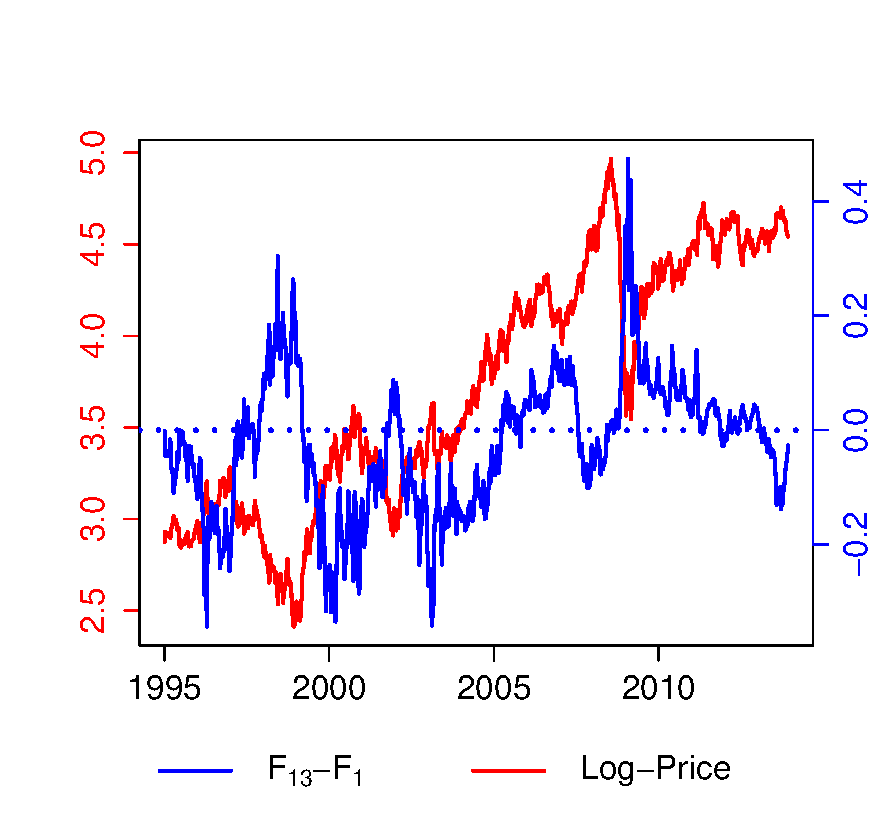
\includegraphics[scale=.6]{LogPrice_TermStructure.eps}
\caption{Log-price (red line) and slope of future curves (blue line)}
\label{fig:LogPriceTermStructure:data}
\end{figure}
%The first regime (in backwardation) is identified by a higher mean-reversion of convenience yield $\alpha$ and a higher volatility in states variables ($\sigma$ and $\eta$). 
%And vice versa the second regime is characterized by a lower value of $\alpha, \sigma, \eta$.
%\begin{verbatim}
%TODO: Add reference: Explain why $rho$ must be high (at least positive).
%TODO: Explain why the noises $g1$, $g4$ are greater than the intermediate contracts
%\end{verbatim}


The correlation between the spot price and the convenience yield is positive and high in both two regimes. The positive correlation verifies one of the fundamental principes in commodity market as in \cite{gibson:schwartz:1990}. That explains when the spot prices are expected to inscrease, the convenience yield are also expected to inscrease. In addition, the higher the correlation is, the more the slope of future curve descreases in function of maturity. It descreases even further in the first regime (in backwardation): the higher volatility higher convenience yield with the higher correlation.


Figure~\ref{fig:posterior:data} and~\ref{fig:posterior:data:logprice} displays the the estimated posterior probabilities of the regime labels and the observed future slope. When the future curve is in backwardation (resp. contango), the model is expected to be in the first regime (resp. second regime), except for the period where the slope of the future curve is too small and in the period from December $2008$ to April $2009$ (beginning of the crisis). 


%After convergence, the value obtained for $\kappa$ is slightly greater than the one obtained in \cite{almansour:2014} but we also obtain slightly lower values for $\eta_1$ and $\eta_2$. The result also shows that the future price of maturity $4W$ is such that $g_4$ is greater than all the other $g_i$'s. It may be explained by the fact that there is no observation of spot contract which is likely to impact mostly the front future contract.


%\begin{figure}
%\centering
%\includegraphics[scale=.38]{alpha_M.png}\\
%\includegraphics[scale=.38]{sigma_M.png}\\
%\includegraphics[scale=.38]{eta_M.png}
%\caption{Estimation of $\alpha$, $\sigma$ and $\eta$.}
%\end{figure}


\begin{figure}
	\centering
	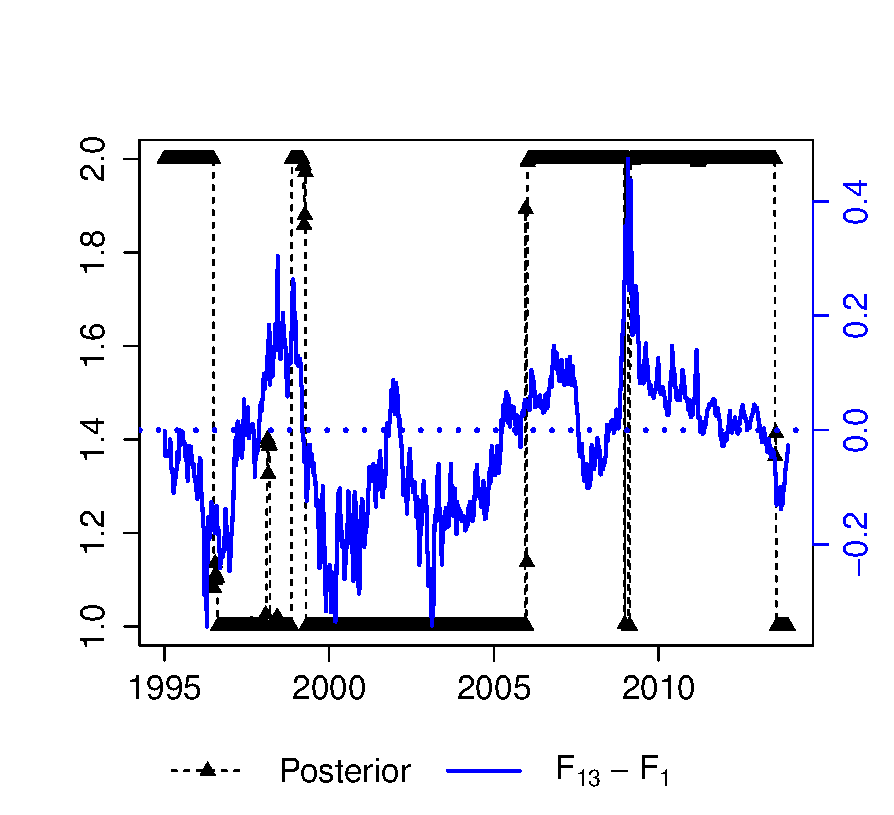
\includegraphics[scale=.6]{Posterior_Data.eps}
	\caption{Posterior probability (triangle black) and slope of future curves (blue line)}
	\label{fig:posterior:data}
\end{figure}

\begin{figure}
	\centering
	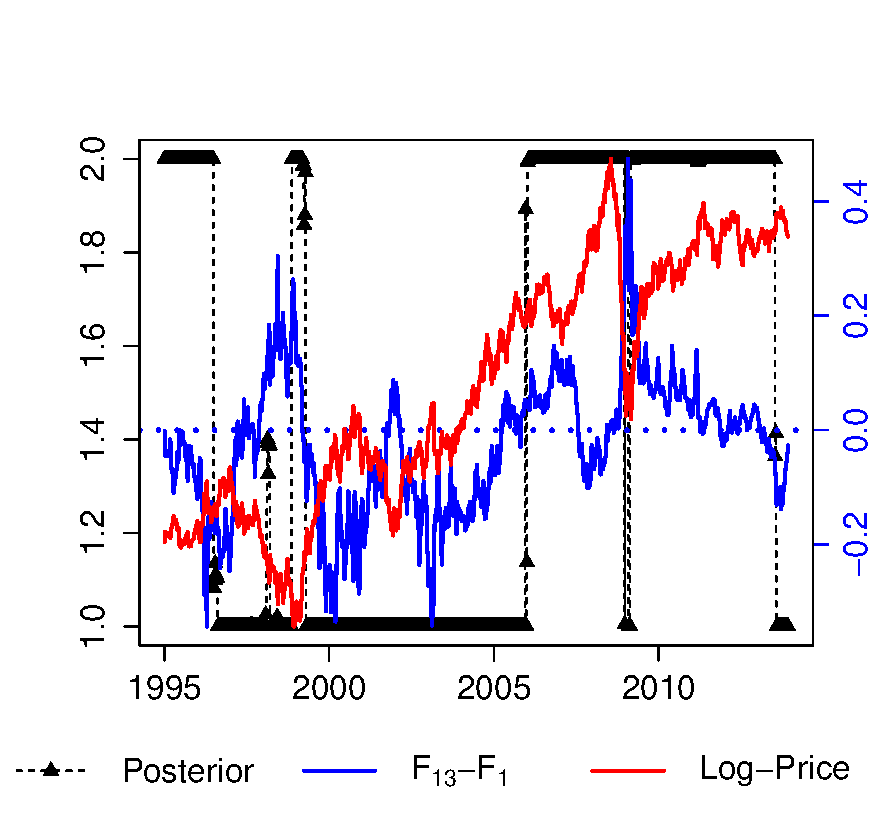
\includegraphics[scale=.75]{Posterior_Data_LogPrice.eps}
	\caption{Posterior probability (triangle black) and slope of future curves (blue line)}
	\label{fig:posterior:data:logprice}
\end{figure}



%\paragraph{Comparaison of estimated future prices with the observations}
%It is interesting to assess the accuracy of the estimated parameters obtained with the EM algorithm. These estimated parameters are used to estimate the future prices and compare them with the observed ones for each maturity. The results of this estimation procedure is displayed in Figure~\ref{fig:density:4W3M} and Figure~\ref{fig:density:6M1Y}.

%\begin{figure*}[htb]
%	\centering
%		\begin{tabular}{||c|c|c|c|c||}
%		Residuals & $F_{4W}$ & $F_{3M}$ & $F_{6M}$ & $F_{1Y}$\\
%		\hline
%		mean & -0.002654812 & 0.001178231 & 0.002130222 & 0.002391526 \\
%		std & 0.01461169 & 0.00575261 & 0.01039791 & 0.01796323
%		\end{tabular}
%	\caption{Table of differences between estimated and observed future prices.}
%	\label{tab:tableTest}
%\end{figure*}
%Mean value of the residuals between the estimated and observed log-future prices are close to $0$ with a small variance. The standard deviation of futures $4W$ has an important value in comparison to futures $3M$ or $6M$ which goes along with the remark for the estimation of $G$ in the equation \eqref{eq:model:obs} by the EM algorithm.

%\FloatBarrier

%Our algorithm is calibrated using future prices of maturities $4W, 3M, 6M$ and $1Y$ but may be used to estimate future prices of maturities $8W, 9M, 2Y, 3Y$. These estimations may be compared to the observations given in the market. Densities of the estimated prices for these others maturities $8W, 9M, 2Y, 3Y$ are shown in Figure~\ref{fig:densothers}.
%\begin{figure}
%\centering
%\includegraphics[scale=.4]{Density_Estim_Obs_OUTSIDE.png}
%\caption{Densities of estimated and observed log-future prices $8W, 9M, 2Y, 3Y$.}
%\label{fig:densothers}
%\end{figure}
%At first glance, mean values and standard deviations of the difference between observed and estimated future prices are greater than in the previous case since these maturities are not used to calibrate the model. Nevertheless, these errors remain close to $0$. In addition, standard deviations of futures $2Y$ and $3Y$ are greater than the ones of $8W$ and $9M$, it is reasonable since $2Y$ and $3Y$ futures are outside of the interval of maturities used to calibrate the model.
%\FloatBarrier


\appendix

\section{Technical lemmas}%~\ref{eq:technical:twofilter}-\ref{lem:integral:gammap}
\begin{lemma}
\label{lem:integratedSDE}
Let $(X_t,\delta_t)_{t\ge0}$ be solutions to the following SDE:
\begin{align*}
\rmd X_t &= \left(\mu - \delta_t- \sigma^2/2 \right) dt + \sigma d W^1_t \eqsp,\\
\rmd \delta_t &= \kappa\left( \alpha - \delta_t\right)dt + \eta dW^2_t \eqsp,
\end{align*}
$(W_t^1)_{t\ge 0}$ and $(W_t^2)_{t\ge 0}$ are standard Brownian motions such that $\rmd \langle W_t^1,W_t^2 \rangle = \rho\rmd t$.
Then, for all $t\ge 0$ and $h>0$,
\[
\begin{pmatrix} X_{t+h} \\ \delta_{t+h}\end{pmatrix} = d_h + T_h\begin{pmatrix} X_{t} \\ \delta_{t}\end{pmatrix} + H_h\varepsilon\eqsp,
\]
where $\varepsilon$ is a standard 2-dimensional Gaussian random variable and (with $\barH_h\eqdef H_h'H_h$),
\[
d \eqdef
\begin{pmatrix} \left[\mu- \alpha - \sigma^2/2 \right] h + \alpha[1-e^{-\kappa h}]/\kappa\\
\alpha [1-e^{-\kappa h}] \end{pmatrix}\eqsp, \;\; T_h \eqdef
\begin{pmatrix} 1 & -[1-e^{-\kappa h}]/\kappa \\ 0 & e^{-\kappa h} \end{pmatrix} \eqsp,
\]
\begin{align*}
\barH_h(1,1) & \eqdef \sigma^2 h+ \eta^2\left\{h + (1-e^{-2\kappa h})/(2\kappa) - 2(1-e^{-\kappa h})/\kappa  \right\}/\kappa^2 \\
&\hspace{7cm} -2\rho\eta\sigma\left\{h - (1-e^{-\kappa h})/\kappa \right\}/\kappa\eqsp, \\
\barH_h(1,2) & \eqdef \left(\rho \eta \sigma-\eta^2/\kappa\right)\left(1-e^{-\kappa h} \right)/\kappa + \eta^2\left(1-e^{-2\kappa h} \right)/(2\kappa^2)\eqsp,\\
\barH_h(2,1) & \eqdef \barH_h(1,2)\eqsp,\\
\barH_h(2,2) & \eqdef \eta^2\left( 1-e^{-2\kappa h} \right)/(2\kappa)\eqsp.
\end{align*}
\end{lemma}

\begin{proof}
For all $t\ge 0$,
\[
X_t = X_0 + (\mu-\sigma^2/2)t - \int_0^t\delta_s\rmd s +\sigma W_t^1
\]
and, as $(\delta_t)_{0\le t\le T}$ is an Ornstein-Uhlenbeck process,
\[
\delta_t = \delta_0\rme^{-\kappa t} + \alpha(1-\rme^{-\kappa t}) + \int_0^t \eta \rme^{\kappa(s-t)}\rmd W^2_s\eqsp.
\]
Then,
\begin{align*}
\int_0^t\delta_s\rmd s &= (\delta_0-\alpha)(1-\rme^{-\kappa t})/\kappa + \alpha t + \eta\int_0^t\int_0^s\rme^{\kappa(u-s)}\rmd W^2_u\rmd s\eqsp,\\
&=(\delta_0-\alpha)(1-\rme^{-\kappa t})/\kappa + \alpha t + (\eta/\kappa) \int_0^t (1-\rme^{-\kappa (t-s)}) \rmd W^2_s\eqsp.
\end{align*}
Defining $\tilde{W}^1_t \eqdef - (\eta/\kappa) \int_0^t (1-\rme^{-\kappa (t-s)}) \rmd W^2_s+\sigma W_t^1$ and $\tilde{W}_t^2\eqdef \int_0^t \eta \rme^{\kappa(s-t)}\rmd W^2_s$, this yields:
\begin{align*}
X_t &= X_0 +  (\mu-\sigma^2/2)t + (\alpha-\delta_0)(1-\rme^{-\kappa t})/\kappa - \alpha t + \tilde{W}_t^1\eqsp,\\
\delta_t &= \delta_0\rme^{-\kappa t} + \alpha(1-\rme^{-\kappa t}) + \tilde{W}^2_t\eqsp.
\end{align*}
The proof is concluded upon noting that $\tilde{W}^1_t$ and $\tilde{W}^2_t$ are centered Gaussian random variables such that:
\begin{itemize}
\item $\!\!\mathrm{Var}\left[\tilde{W}^1_t\right] = \sigma^2  t + \eta^2\left\{ t + (1-e^{-2\kappa t})/(2\kappa) - 2(1-e^{-\kappa  t})/\kappa\right\}/\kappa^2 - 2\rho \eta \sigma\left\{ t - (1-e^{-\kappa  t})/\kappa \right\}/\kappa\eqsp,$
\item $\!\!\mathrm{Var}\left[\tilde{W}^2_t\right] = \eta^2(1-\rme^{-2\kappa t})/(2\kappa)\eqsp,$
\item $\!\!\mathrm{Cov}\left[\tilde{W}^1_t,\tilde{W}^2_t\right] = \left(\rho \eta\sigma-\eta^2/\kappa\right)\left(1-e^{-\kappa t} \right)/\kappa + \eta^2 \left(1-e^{-2\kappa t} \right)/(2\kappa^2)\eqsp.$
\end{itemize}
\end{proof}

\label{sec:app:proofs}
Lemmas~\ref{eq:technical:twofilter}, \ref{lem:py} and \ref{lem:integral:gammap} are close to \cite[Proposition 5, Proposition 6]{briers:doucet:maskell:2010}. The proofs are detailed in this appendix for completeness.
\begin{proof}[Proof of Lemma~\ref{eq:technical:twofilter}]
For all $1\le i \le n-1$,
\begin{align*}
p_{}(y_{i:n}|a_i,z_i) &= \sum_{a_{i+1:n}}\int p_{}(y_{i:n},a_{i+1:n},z_{i+1:n}|a_i,z_i)\rmd z_{i+1:n}\eqsp,\\
&=  \sum_{a_{i+1:n}}\int p_{}(a_{i+1:n},z_{i+1:n}|a_i,z_i)p_{}(y_{i:n}|a_{i:n},z_{i:n})\rmd z_{i+1:n}\eqsp,\\
&=  \frac{\tilde{p}_{i}(y_{i:n})}{\gamma^{}_{i}(a_i,z_i)}\sum_{a_{i+1:n}}\int \frac{\gamma^{}_{i}(a_i,z_i)}{\tilde{p}_{i}(y_{i:n})}p_{}(a_{i+1:n},z_{i+1:n}|a_i,z_i)p_{}(y_{i:n}|a_{i:n},z_{i:n})\rmd z_{i+1:n}\eqsp,\\
&=  \frac{\tilde{p}_{i}(y_{i:n})}{\gamma^{}_{i}(a_i,z_i)}\sum_{a_{i+1:n}}\int \tilde{p}_{i}(a_{i:n},z_{i:n}|y_{i:n})\rmd z_{i+1:n}\eqsp,\\
&=  \frac{\tilde{p}_{i}(y_{i:n})}{\gamma^{}_{i}(a_i,z_i)}\tilde{p}_{i}(a_{i},z_{i}|y_{i:n})\eqsp,
\end{align*}
which concludes the proof of \eqref{eq:p:y1:n}. To prove \eqref{eq:p:ai:zi} write,
\begin{align*}
\tilde{p}_{i}(a_{i:n},z_{i}|y_{i:n}) &= \frac{\gamma^{}_{i}(a_i,z_i)}{\tilde{p}_{i}(y_{i:n})}\int p_{}(y_{i:n}|a_{i:n},z_{i:n})p_{}(a_{i+1:n},z_{i+1:n}|a_{i},z_{i})\rmd z_{i+1:n}\eqsp,\\
&= \frac{\gamma^{}_{i}(a_i,z_i)}{\tilde{p}_{i}(y_{i:n})}\int \frac{p_{}(y_{i:n}|a_{i:n},z_{i})p_{}(z_{i+1:n}|y_{i:n},a_{i:n},z_i)}{p_{}(z_{i+1:n}|a_{i:n},z_i)}p_{}(a_{i+1:n},z_{i+1:n}|a_{i},z_{i})\rmd z_{i+1:n}\eqsp,\\
&=\frac{\gamma^{}_{i}(a_i,z_i)}{\tilde{p}_{i}(y_{i:n})}p_{}(y_{i:n}|a_{i:n},z_{i})p_{}(a_{i+1:n}|a_i)\eqsp.
\end{align*}
Therefore,
\[
\tilde{p}_{i}(a_{i},z_{i}|y_{i:n}) = \frac{\gamma^{}_{i}(a_i,z_i)}{\tilde{p}_{i}(y_{i:n})}\sum_{a_{i+1:n}}p_{}(y_{i:n}|a_{i:n},z_{i})p_{}(a_{i+1:n}|a_i)
\]
and the proof is completed upon noting that
\[
\tilde{p}_{i}(a_{i:n}|y_{i:n}) = \frac{p_{}(a_{i+1:n}|a_i)}{\tilde{p}_{i}(y_{i:n})} \int \gamma^{}_{i}(a_i,z)p_{}(y_{i:n}|a_{i:n},z)\rmd z\eqsp.
\]
\end{proof}

\begin{proof}[Proof of Lemma~\ref{lem:py}]
The result is proved by backward induction. \eqref{eq:cn}, \eqref{eq:Pn} and \eqref{eq:nun} follow directly from \eqref{eq:model:obs}. Assume that for a given $1\le i\le n-1$, $p(y_{i+1:n}|a_{i+1:n},z_{i+1})$ is given by \eqref{eq:py}. Write
\[
p(y_{i:n}|a_{i:n},z_i) = \int p(z_{i+1}|z_i,a_{i+1})p(y_i|z_i,a_i)p(y_{i+1:n}|a_{i+1:n},z_{i+1})\rmd z_{i+1}\eqsp,
\]
with
\begin{align*}
p(z_{i+1}|z_i,a_{i+1}) &= \exp\left\{-\frac{\dimz}{2}\log(2\pi)-\frac{1}{2}\log|\barH_{a_{i+1}}|-\frac{1}{2}\normMat{\barH_{a_{i+1}}}{z_{i+1}-d_{a_{i+1}}-T_{a_{i+1}}z_i}^2\right\}\eqsp,\\
p(y_i|z_i,a_i)& = \exp\left\{-\frac{\dimy}{2}\log(2\pi)-\frac{1}{2}\log|\barG_{a_i}|-\frac{1}{2}\normMat{\barG_{a_i}}{y_{i}-c_{a_{i}}-B_{a_i}z_i}^2\right\}\eqsp,\\
p(y_{i+1:n}|a_{i+1:n},z_{i+1})& = \exp\left\{-\frac{1}{2}c_{i+1}(a_{i+1:n}) - \frac{1}{2}\normMat{\tilde{P}_{i+1}(a_{i+1:n})}{z_{i+1}}^2 + z'_{i+1}\tilde{\nu}_{i+1}(a_{i+1:n})\right\}\eqsp.
\end{align*}
Let $\Delta_{i}$ and  $\delta_{i}$ be given by:
\begin{align*}
\Delta_{i}(a_{i+1:n}) &\eqdef \left(I_{\dimz} + H'_{a_{i+1}}\tilde{P}_{i+1}^{-1}(a_{i+1:n})H_{a_{i+1}}\right)^{-1}\eqsp,\\
\delta_{i}(a_{i+1:n}) &\eqdef \nu_{i+1}(a_{i+1:n}) + \barH_{a_{i+1}}^{-1}(d_{a_{i+1}}+T_{a_{i+1}}z_i)\eqsp.
\end{align*}
Then, $\barH_{a_{i+1}}^{-1} + \tilde{P}_{i+1}^{-1}(a_{i+1:n}) = \left(H_{a_{i+1}}\Delta_{i}(a_{i+1:n})H'_{a_{i+1}}\right)^{-1}$ and \eqref{eq:ck}, \eqref{eq:Pk} and \eqref{eq:nuk} follows from
\begin{multline*}
\int \exp\left\{-\frac{1}{2}\normMat{H_{a_{i+1}}\Delta_{i}(a_{i+1:n})H'_{a_{i+1}}}{z_{i+1}}^2 + z'_{i+1}\delta_{i}(a_{i+1:n})\right\}\rmd z_{i+1}\\
 =\exp\left\{\frac{1}{2}\log(2\pi) + \frac{1}{2}\log|H_{a_{i+1}}\Delta_{i}(a_{i+1:n})H'_{a_{i+1}}|+\frac{1}{2}\delta'_{i}(a_{i+1:n})'H_{a_{i+1}}\Delta_{i}(a_{i+1:n})H'_{a_{i+1}}\delta_{i}(a_{i+1:n})\right\}\eqsp.
\end{multline*}
\end{proof}

\begin{proof}[Proof of Lemma~\ref{lem:integral:gammap}]
By Lemma~\ref{lem:py},
\begin{multline*}
\phi_{\mu_i,\Sigma_i}(z_i)p(y_{i:n}|a_{i:n},z_i) = \exp\left\{-\frac{\dimz}{2}\log(2\pi) -\frac{1}{2}\log|\Sigma_i|-\frac{1}{2}\normMat{\Sigma_i}{z_i-\mu_i}^2\right\}\\
\times\exp\left\{-\frac{1}{2}c_{i}(a_{i:n})-\frac{1}{2}\normMat{\tilde{P}_{i}(a_{i:n})}{z_i}^2+z'_i\nu_{i}(a_{i:n})\right\}\eqsp.
\end{multline*}
The proof is completed noting that
\begin{multline*}
\int \exp\left\{-\frac{1}{2}z'_i\tilde{\Omega}_{i}^{-1}(a_{i:n})z_i + z'_i(\Sigma_i^{-1}\mu_i+\nu_{i}(a_{i:n}))\right\}\rmd z_{i}\\
= \exp\left\{\frac{\dimz}{2}\log(2\pi) + \frac{1}{2}\log|\tilde{\Omega}_{i}(a_{i:n})| +\frac{1}{2}\left[\Sigma_i^{-1}\mu_i+\nu_{i}(a_{i:n})\right]'\tilde{\Omega}_{i}(a_{i:n})\left[\Sigma_i^{-1}\mu_i+\nu_{i}(a_{i:n})\right]\right\}\eqsp.
\end{multline*}
\end{proof}

%\clearpage
%\newpage
%
%\section{Algorithms}
%The forward filter is described in Algorithm~\ref{algo:forward}. The conditional distribution of $Y_i$ given $a^k_{1:i-1}$, $a_i$ and $Y_{1:i-1}$ is a Gaussian distribution with mean $c_{a_i}+B_{a_i}\mu^k_{i|i-1}$ and variance $B_{a_i}P^k_{i|i-1}B'_{a_i} + \barG_{a_i}$ which means that $\gamma_i^j$ may be written:
%\begin{align*}
%\gamma_i^j &= p(y_i | a_i = j, a_{1:i-1}^k, y_{1:i-1}) Q(a_{i-1}^k,j) \eqsp, \\
%& =  Q(a_{i-1}^k,j)|B_jP^k_{i|i-1}B'_j + \barG_j|^{-1/2}\exp\left\{-\frac{1}{2}\normMat{B_jP^k_{i|i-1}B'_j + \barG_j}{y_i-c_{j}-B_j\mu^k_{i|i-1}}^2\right\} \eqsp.
%\end{align*}
%\begin{algorithm}
%\DontPrintSemicolon
%\KwIn{Initial distribution $\pi$ on $\{1,\ldots,J\}$, initial mean $\mu_1$ and variance $\Sigma_1$.}
%\KwOut{A set of trajectories $(a^k_{1:i})_{1\le k\le N}$, means $(\mu^k_{i})_{1\le k\le N}$ and variances $(P^k_{i})_{1\le k\le N}$ with importance weights $(\omega^k_i)_{1\le k\le N}$, $1\le i \le n$.}
%{\bf Initialization}\;
%\For{$k \gets 1$ \textbf{to} $N$} {
%Sample $a^k_1 \in \{1,\ldots,J\}$ such that $\mathbb{P}\left(a_1^k = j\right) = \pi_j$. \;
%Compute $\mu_1^k$ and $P_1^k$:
%\begin{align*}
%K^k_{1} &=\Sigma_1B'_{a_1^k}\left(B_{a_1^k}\Sigma_1B'_{a_1^k} + \barG_{a_1^k}\right)^{-1}\eqsp,\\
%\mu^k_{1} &= \mu_{1} + K^k_1\left(Y_1 - c_{a_{1}^k} - B_{a_1^k}\mu_{1}\right)\eqsp,\\
%P^k_{1} &=\left(I-K^k_{1}B_{a_1^k}\right)\Sigma_1\eqsp.
%\end{align*}
%Update the importance weight: $\omega^k_1 \propto p(y_1|a_1^k)$.
%}
%{\bf Iterations}\;
%\For{$i \gets 2$ \textbf{to} $n$} {
%Resample the set $(\{a^k_{1:i-1}, \mu^k_{i-1}, P^k_{i-1}\})_{1\le k\le N}$ using the normalized weights $(\omega^k_{i-1})_{1\le k \le N}$.\;
%\For{$k \gets 1$ \textbf{to} $N$} {
%For all $j \in \{1,\ldots, J\}$ compute
%\[
%\gamma_i^{j,k} = p(y_i | a_i = j, a_{1:i-1}^k, y_{1:i-1}) q(a_{i-1}^k,j)\eqsp.
%\]
%Sample $a_i^k \in \{1,\ldots, J\}$ using the normalized weights $(\gamma_i^{j,k})_{1\le j\le J}$.\;
%Update $\mu_i^k$ and $P_i^k$:
%\begin{align*}
%\mu^{k}_{i|i-1} &= d_{a_{i}^k} + T_{a_{i}^k}\mu^k_{i-1}\eqsp,\\
%P^k_{i|i-1} &= T_{a_{i}^k}P^k_{i-1}T'_{a_{i}^k} + \barH_{a_{i}^k}\eqsp,\\
%K^k_{i} &=P^k_{i|i-1}B'_{a_{i}^k}\left(B_{a_{i}^k}P^k_{i|i-1}B'_{a_{i}^k} + \barG_{a_{i}^k}\right)^{-1}\eqsp,\\
%\mu^k_{i} &= \mu^{k}_{i|i-1} + K^k_i\left(Y_i - c_{a_{i}^k} - B_{a_{i}^k}\mu^{k}_{i|i-1}\right)\eqsp,\\
%P^k_{i} &=\left(I-K^k_{i}B_{a_{i}^k}\right)P^k_{i|i-1}\eqsp.
%\end{align*}
%Update the importance weights: $\omega_i^k \propto \sum_{j=1}^J \gamma_i^{j,k}$.
%}
%}
%\caption{Forward filter, see \cite{chen:liu:2000}}
%\label{algo:forward}
%\end{algorithm}
%
%\begin{algorithm}
%\DontPrintSemicolon
%\KwIn{Output of a forward filter: trajectories $(a^k_{1:i})_{1\le k\le N}$, means $(\mu^k_{i})_{1\le k\le N}$ and variances $(P^k_{i})_{1\le k\le N}$ with importance weights $(\omega^k_i)_{1\le k\le N}$, $1\le i \le n$, .}
%\KwOut{Trajectory $\tilde{a}_{1:n}$ approximatively distributed according to $p(a_{1:n}|y_{1:n})$.}
%{\bf Initialization}\;
%Set $\tilde{a}_n = a_n^k$ with probability $\omega_n^k$.\\
%{\bf Iterations}\;
%\For{$i \gets n-1$ \textbf{to} $1$} {
%\For{$k \gets 1$ \textbf{to} $N$} {
%Compute
%\[
%\omega^k_{i|n} \propto \omega_i^kQ(a_i^k,\tilde{a}_{i+1})\eqsp.
%\]
%}
%Set $\tilde{a}_i = a_i^k$ with probability $\omega_{i|n}^k$.
%}
%\caption{Smoothing algorithm based on the approximation of \cite{kim:1994}}
%\label{algo:kim}
%\end{algorithm}
%
%
%\begin{algorithm}
%\DontPrintSemicolon
%\KwIn{Output of a forward filter: trajectories $(a^k_{1:i})_{1\le k\le N}$, means $(\mu^k_{i})_{1\le k\le N}$ and variances $(P^k_{i})_{1\le k\le N}$ with importance weights $(\omega^k_i)_{1\le k\le N}$, $1\le i \le n$, .}
%\KwOut{Trajectory $\tilde{a}_{1:n}$ approximatively distributed according to $p(a_{1:n}|y_{1:n})$.}
%{\bf Initialization}\;
%Set $\tilde{a}_n = a_n^k$ with probability $\omega_n^k$.\\
%Compute $\hat{\Omega}_n$ and $\hat{\lambda}_n$:
%\[
%\hat{\Omega}_n = B'_{\tilde{a}_n}\barG^{-1}_{\tilde{a}_n}B_{\tilde{a}_n}\quad\mbox{and}\quad \hat{\lambda}_n =B'_{\tilde{a}_n}\barG^{-1}_{\tilde{a}_n}(y_n-c_{\tilde{a}_n})\eqsp.
%\]
%{\bf Iterations}\;
%\For{$i \gets n-1$ \textbf{to} $1$} {
%Compute 
%\[
%m_{i+1} = \hat{\lambda}_{i+1} - \hat{\Omega}_{i+1}d_{\tilde{a}_{i+1}}\quad\mbox{and}\quad M_{i+1} = H_{\tilde{a}_{i+1}}'\hat{\Omega}_{i+1}H_{\tilde{a}_{i+1}} + I\eqsp.
%\]
%Set
%\begin{align*}
%\Omega_i &= T'_{\tilde{a}_{i+1}}(I-\hat{\Omega}_{i+1}H_{\tilde{a}_{i+1}}M^{-1}_{i+1}H'_{\tilde{a}_{i+1}})\hat{\Omega}_{i+1}T_{\tilde{a}_{i+1}}\eqsp,\\
%\lambda_i &=T'_{\tilde{a}_{i+1}}(I-\hat{\Omega}_{i+1}H_{\tilde{a}_{i+1}}M^{-1}_{i+1}H'_{\tilde{a}_{i+1}})m_{i+1}\eqsp.
%\end{align*}
%\For{$k \gets 1$ \textbf{to} $N$} {
%Compute
%\[
%\Lambda^k_i = (\Gamma_i^k)'\Omega_i\Gamma_i^k + I \quad\mbox{and}\quad \eta^k_i = \|\mu_i^k\|^2_{\Omega^{-1}_i} - 2\lambda'_i\mu_i^k-\|(\Gamma_i^k)'(\lambda_i-\Omega_i\mu_i^k)\|^2_{\Lambda_i}\eqsp.
%\]
%Set
%\[
%\tilde{\omega}_{i|n}^k \propto \omega_i^kQ(a_i^k,\tilde{a}_{i+1})|\Lambda^k_i|^{-1/2}\exp\left\{\eta^k_i/2\right\}\eqsp.
%\]
%}
%Set $\tilde{a}_i = a_i^k$ with probability $\omega_{i|n}^k$ and
%\[
%\hat{\Omega}_i =  \Omega_i + B'_{\tilde{a}_i}\barG^{-1}_{\tilde{a}_i}B_{\tilde{a}_i} \quad\mbox{and}\quad \hat{\lambda}_i = \lambda_i + B'_{\tilde{a}_i}\barG^{-1}_{\tilde{a}_i}(y_i-c_{\tilde{a}_i})\eqsp.
%\]
%}
%\caption{FFBS based algorithm of \cite{lindsten:bunch:sarkka:schon:godsill:2015}}
%\label{algo:FFBS}
%\end{algorithm}
%
%
%\begin{algorithm}[b]
%\DontPrintSemicolon
%\KwIn{Artificial densities $(\gamma^{}_i)_{1\le i\le n}$ and proposal densities $(\tilde{q}_i)_{1\le i \le n}$.}
%\KwOut{A set of weighted trajectories $(\tilde{a}^j_{i:n})_{1\le j\le N}$ with importance weights $(\tilde{\omega}^j_i)_{1\le j\le N}$, $1\le i \le n$.}
%{\bf Initialization}\;
%For $1\le \ell \le N$, sample $\tilde{a}^{\ell}_n\sim\tilde{q}_n(\cdot)$.\;
%For $1\le \ell \le N$, set:
%\[
%\tilde{\omega}^{\ell}_n \propto \frac{\int\gamma^{}_n(\tilde{a}^{\ell}_n,z')g_{}(\tilde{a}^{\ell}_n,z';y_n)\rmd z'}{\tilde{q}_n(\tilde{a}^{\ell}_n)}\eqsp.
%\]
%{\bf Iterations}\;
%\For{$i \gets n-1$ \textbf{to} $1$} {
%Resample the set $(\tilde{a}^{\ell}_{i+1:n})_{1\le j\le N}$ using the normalized weights $(\tilde{\omega}^{\ell}_{i+1})_{1\le j \le N}$.\;
%For $1\le \ell \le N$, sample $\tilde{a}^{\ell}_{i}\sim\tilde{q}_i(\tilde{a}^{\ell}_{i+1:n},\cdot)$.\;
%For $1\le \ell \le N$, set:
%\[
%\tilde{\omega}^{\ell}_i \propto \frac{q(\tilde{a}^{\ell}_i,\tilde{a}^{\ell}_{i+1})\int \gamma^{}_i(\tilde{a}^{\ell}_i,z')p_{}(y_{i:n}|\tilde{a}^{\ell}_{i:n},z')\rmd z'}{\tilde{q}_i(\tilde{a}^{\ell}_{i+1:n},\tilde{a}^{\ell}_i)\int \gamma^{}_{i+1}(\tilde{a}^{\ell}_{i+1},z')p_{}(y_{i+1:n}|\tilde{a}^{\ell}_{i+1:n},z')\rmd z'}\eqsp.
%\]
%}
%\caption{Backward information filter, see \cite[Section~4.1.1]{briers:doucet:maskell:2010}}
%\label{algo:backward}
%\end{algorithm}

\bibliographystyle{alpha}

\bibliography{./clgm_bib}
\end{document} 